\documentclass{ttp}

%--------------------------------------------- Basic packages (could be expanded by author)%
\usepackage{floatrow}
%\usepackage{graphicx,wrapfigure}
\usepackage{graphicx}
\usepackage[intlimits]{amsmath}
\usepackage{amssymb}
\usepackage{exscale}
\usepackage{hyperref}
\usepackage{times}
%\usepackage{xparse}
\usepackage{fontspec}
%\ifdefined\directlua
%  \usepackage{fontspec}
%\else
%  \usepackage[T1]{fontenc}
%  \usepackage[nomath]{lmodern}
%\fi
%Для пришвидшення компіляції закоментив \usepackage{subfigure}
%\usepackage{subfigure}
%\usepackage{fontspec-patches}	
	% <-- DO NOT REMOVE this package,
				%       because the fonts (Times New Roman and Arial) will not be used in the document.
					% 	   If you don`t have this package, you can get it from the Internet or you can get this
					%       package from the archive The_Fontspec_package.zip which you downloaded with
					%       this current file.

%---------------------------------------------If you need include the .eps files, please uncomment the package bellow.%
%\usepackage{epsfig}

%--------------------------------------------- Override fonts to Times New Roman and Arial%
\renewcommand{\large}{\fontsize{14}{18pt}\selectfont}
\renewcommand{\small}{\fontsize{11}{13.6pt}\selectfont}
\setmainfont{Times New Roman}
\setsansfont{Arial}

%--------------------------------------------- New commands for quick editing of the document%
\newcommand{\titleformat}{\sffamily\bfseries \large}						%	<--- Doc. title
\newcommand{\authorformat}{\sffamily \large}							%	<--- Authors
\newcommand{\keywordsformat}{\noindent \small \sffamily}				%	<--- Kyewords
\newcommand{\abstractformat}{\noindent \textbf}						%	<--- Abstract
\newcommand{\contentformat}{\rmfamily \normalsize\vspace{18pt}}			%	<--- Main content
\newcommand{\email}{\sffamily \small \vspace{-8pt}}						%	<--- E-mail
\renewcommand{\subsection}{\textbf}	

%--------------------------------------------- Make all internal and external links - black color%
\hypersetup{
    colorlinks,%
    citecolor=black,%
    filecolor=black,%
    linkcolor=black,%
    urlcolor=black
}

%--------------------------------------------- Set the basic parameters of the page. DO NOT CHANGE!%
\special{papersize=210mm,297mm}
\textheight=25.6cm

%--------------------------------------------- For the Publisher to Enter:

\begin{document}

\title{\titleformat Variability in FeB Pair Association Rates in Silicon under Ultrasound Loading: Effects of Acoustic Wave Types}

%\author{ FULL First Author \inst{1}$^{,\rm{a}}$ \textbf{,} FULL Second Author \inst{2}$^{,\rm{b}}$ and Last Author \inst{3}$^{,\rm{c}}$}
\author{\authorformat OLIKH Oleg \inst{1}$^{,\rm{a}}$ and ARUTYUNOV Nikolay \inst{,2,3}$^{,\rm{b}}$}

\institute{\sffamily Department of General Physics, Taras Shevchenko National University of Kyiv, Kyiv, Ukraine
\and Department of Physics, Martin Luther University Halle, Halle, Germany
\and Leibniz-lnstitut für Kristallzüchtung (IKZ), Berlin, Germany}

\maketitle

\begin{center}
\email{ $^{\rm a}$olegolikh@knu.ua, $^{\rm b}$n\_arutyunov@yahoo.com}
%\email{ $^{\rm a}$olegolikh@knu.ua, $^{\rm b}$n_arutyunov@yahoo.com}
\end{center}


\keywordsformat{{\textbf{Keywords:}}  Ultrasound, Silicon, Iron-boron pair, Point defect, Acousto-defect interaction, Positron annihilation
spectroscopy.}

\contentformat

\abstractformat{Abstract.} This template explains and demonstrates how to prepare your camera-ready paper for
\textit {Trans Tech Publications}. The best is to read these instructions and follow the outline of this text.
Please make the page settings of your word processor to A4 format (21 x 29,7 cm or 8~x~11 inches);
with the margins: bottom 1.5 cm (0.59 in) and top 2.5 cm (0.98 in), right/left margins must be 2 cm (0.78 in).
\textbf{(We shall be able to publish your paper in electronic form on our web page }{\url{http://www.scientific.net}}
\textbf{ if the paper format and the margins are correct. If not, we will have to scan your paper which, when compared
with an electronic version, results in very poor quality)}\par
\noindent {Your manuscript will be reduced by approximately 20\% by the publisher. Please keep this in mind when designing your figures and tables etc.}

\section{Introduction}\label{S1}
\vspace{-6pt}

All manuscripts must be in English,


\section{Features of FeB Pair Association under Ultrasonic Loading}

\noindent \textbf{Experiment details.}The section



\noindent \textbf{Results of Acousto-induced Changes in Fe Ion Migration.}

\thisfloatsetup{capposition=beside,%
      capbesideposition={right,top},
      capbesidewidth= 0.5\textwidth,
      floatwidth= 0.45\linewidth
  }


\begin{figure}
	\centering
%     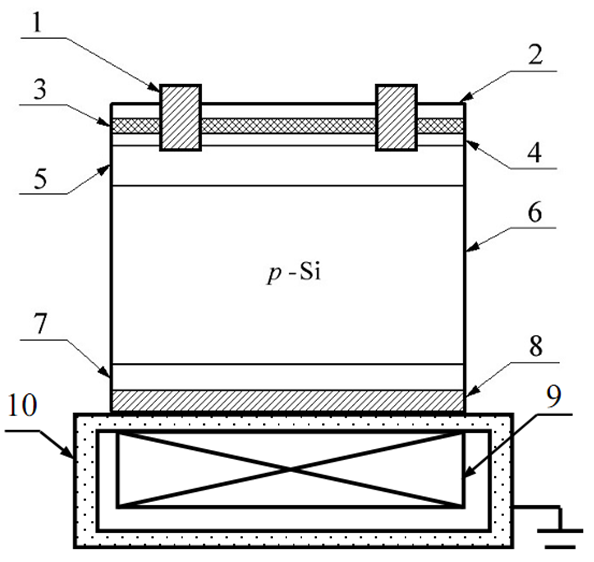
\includegraphics[width=0.45\linewidth]{Fig1.png}
     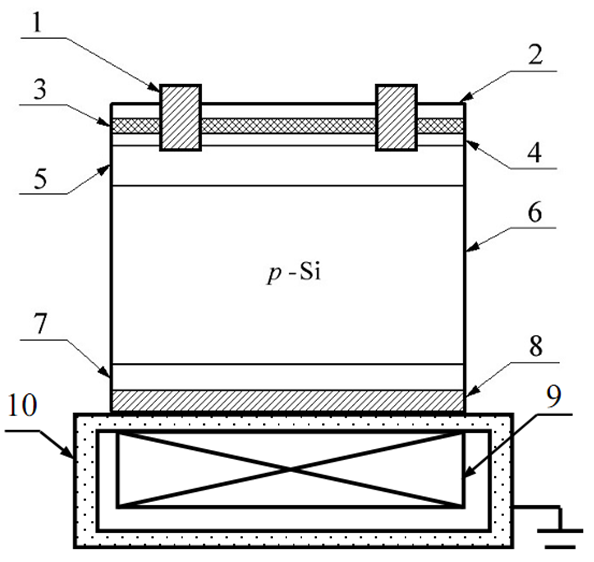
\includegraphics[width=\linewidth]{Fig1.png}
	  \caption{Measured short circuit current plotted as a function of the time after FeB decay
      without USL (1, 3, 5, empty black marks) and under USL (2, 4, 6. filled red marks).
      $T$, K: 300 (1, 2), 320 (3, 4), 340 (5, 6).
      The values of $\tau_\mathrm{ass}^0$ and $\tau_\mathrm{ass}^\mathrm{US}$ obtained 
      by the methodology described in \cite{Olikh2021JAP,Olikh2022:JMatSci} are shown also.
}\label{fig1}
\end{figure}


\begin{figure}
	\centering
     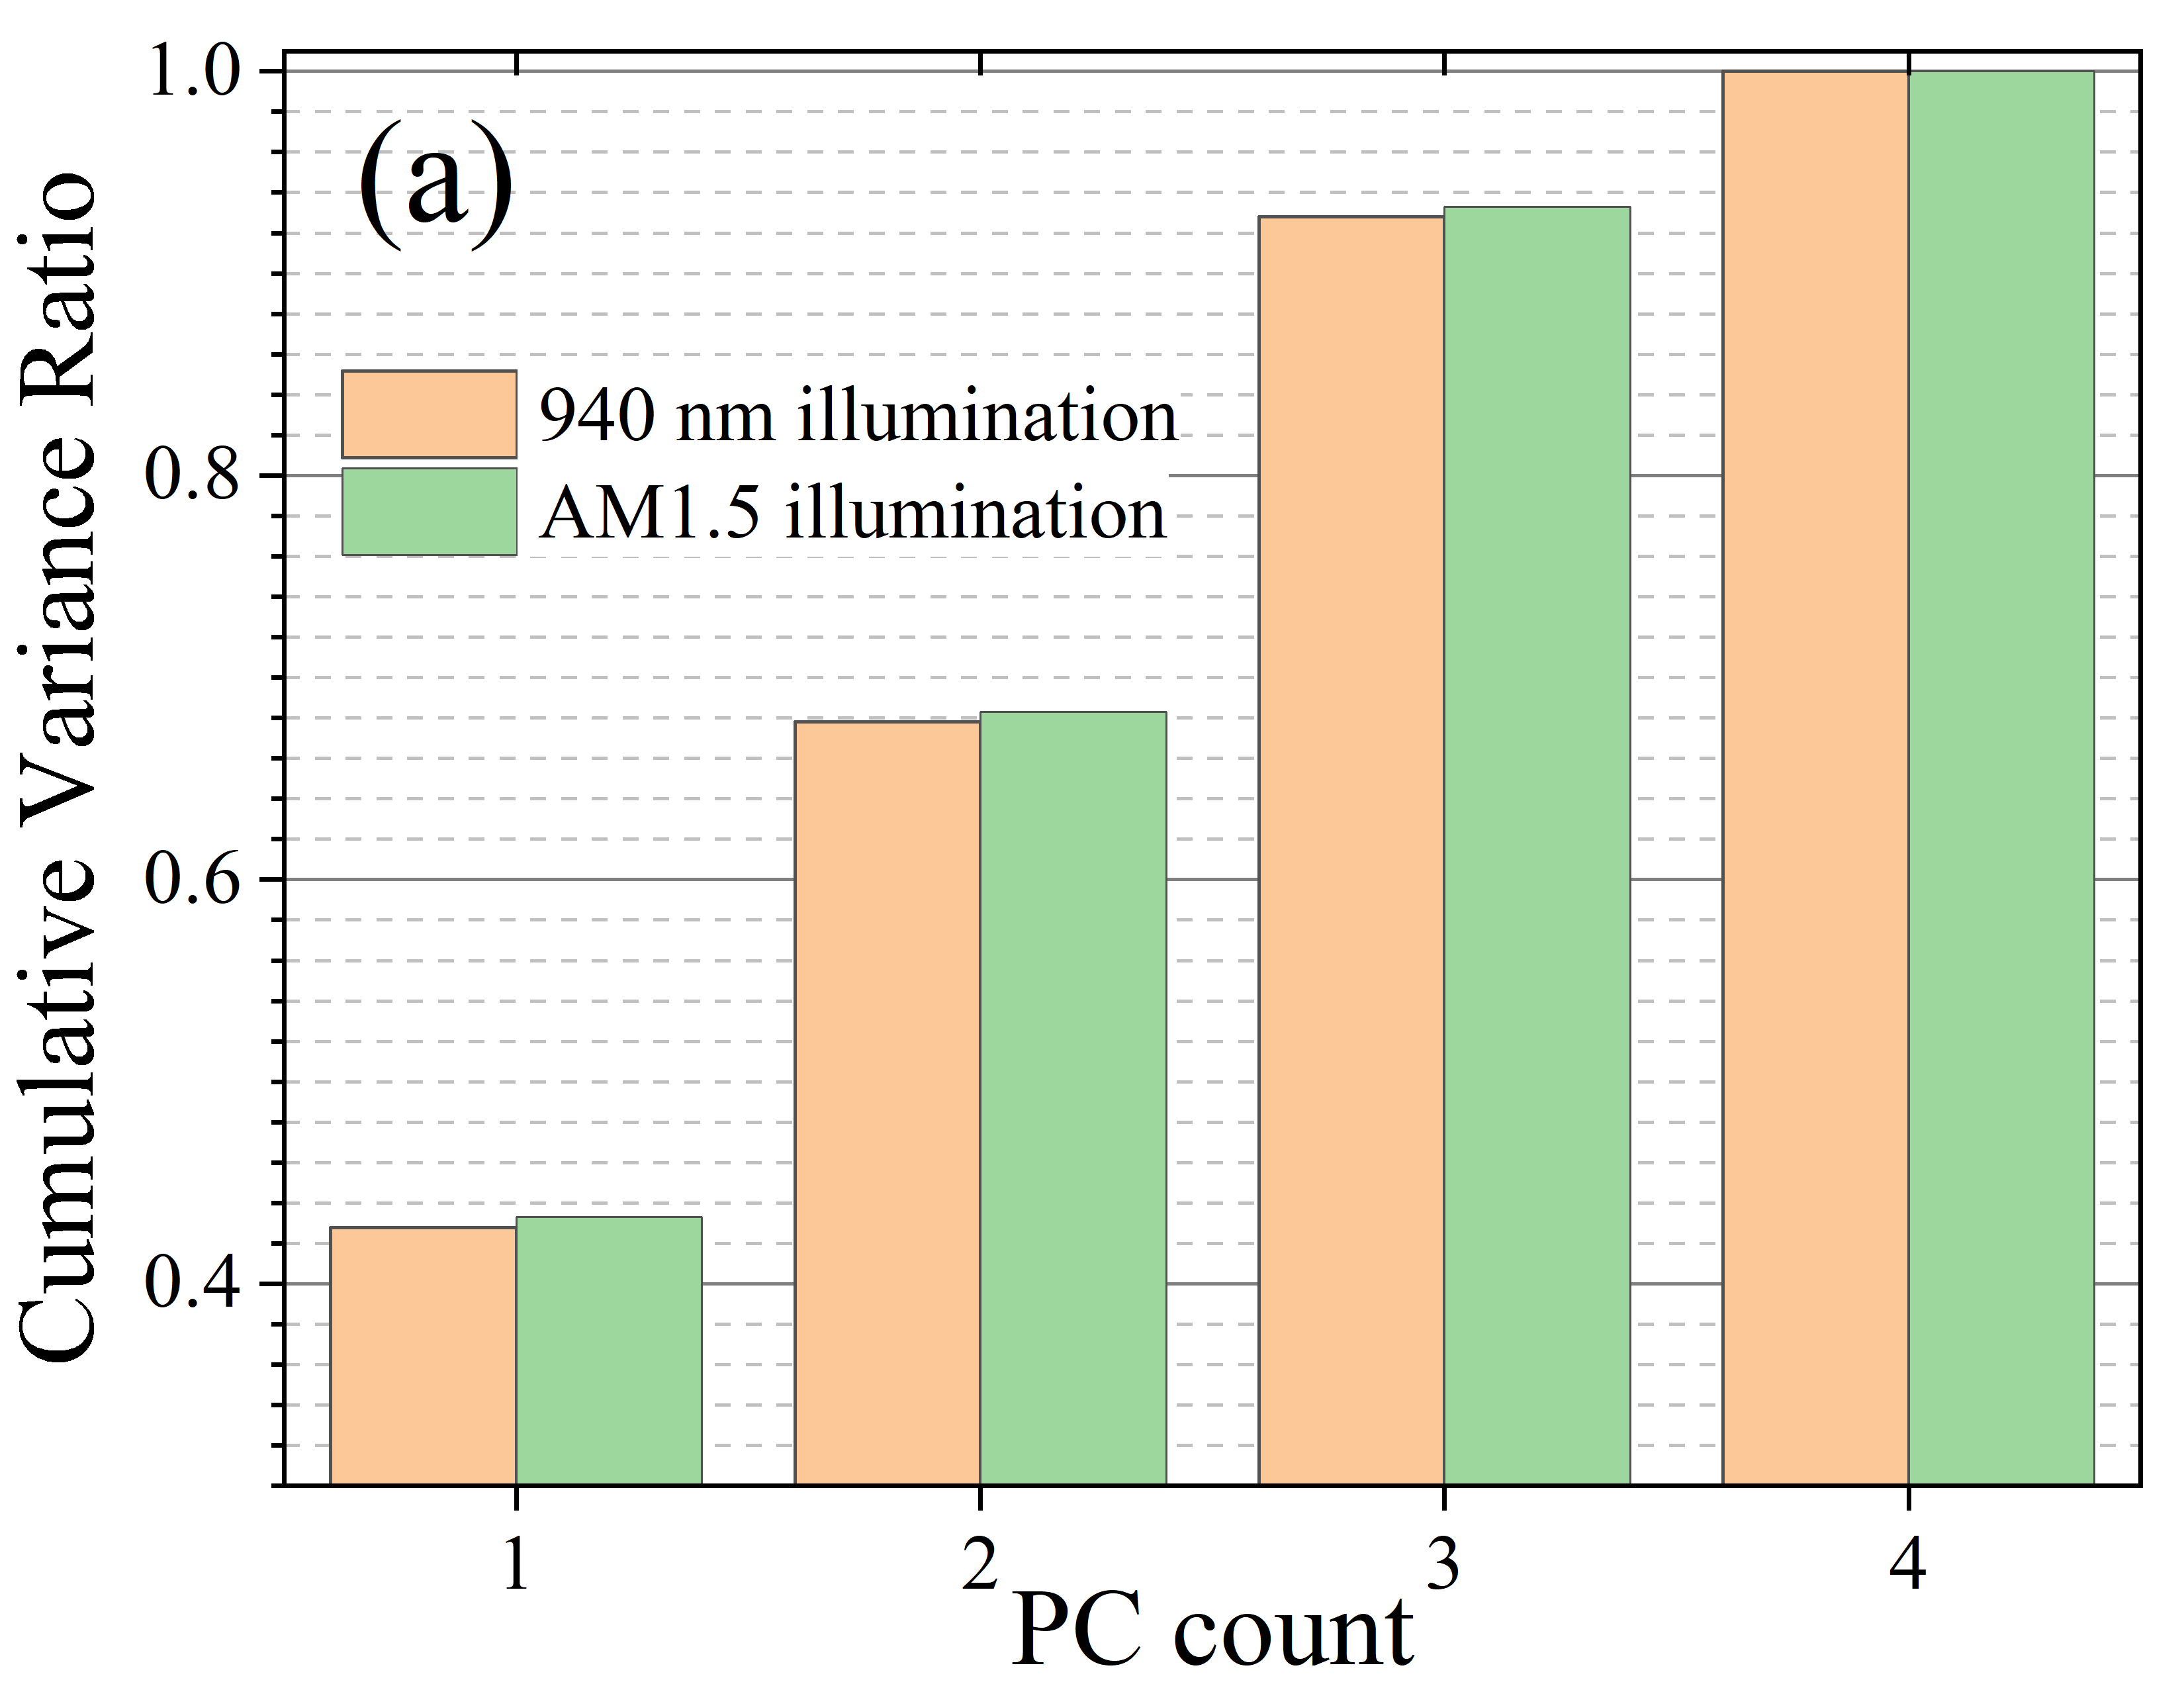
\includegraphics[width=0.4\linewidth]{Fig2a.png}
     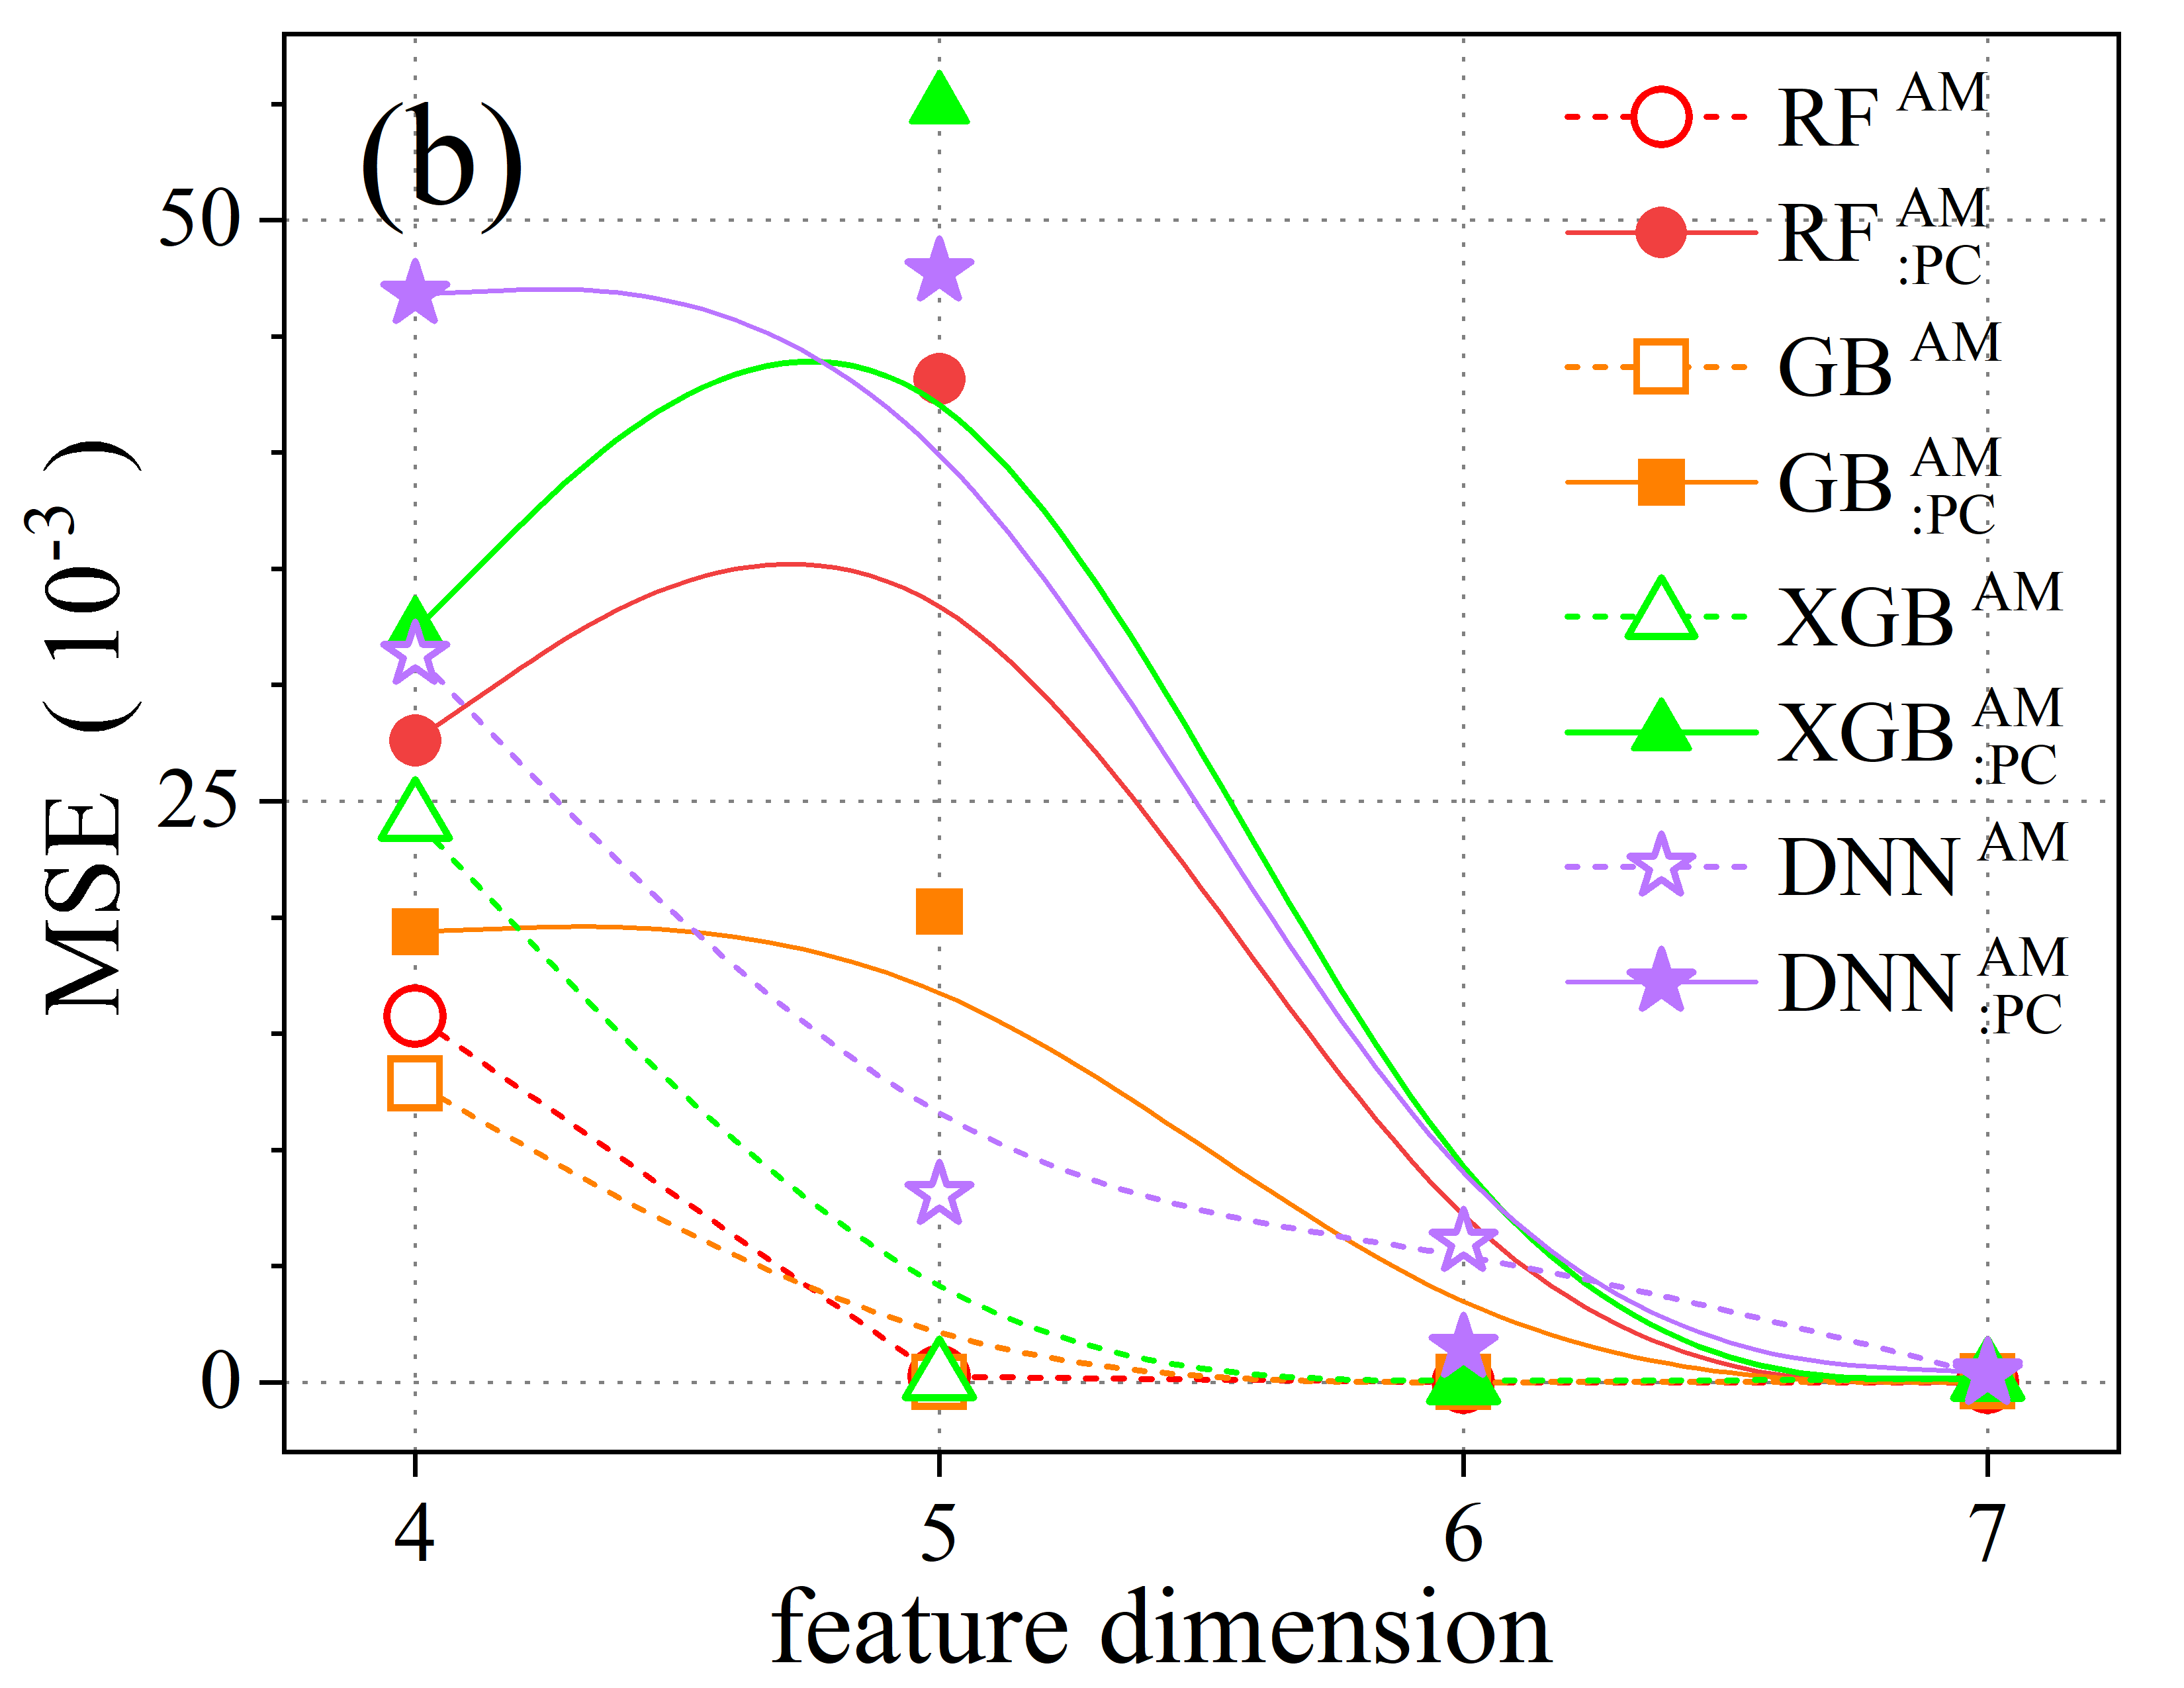
\includegraphics[width=0.4\linewidth]{Fig2b.png}
	  \caption{Dependencies of AI change in migration energy on US intensity for 
       samples with different  iron concentrations.
       $f_\mathrm{US}$, MHz: 5.40 (a), 5.23 (b). 
       AW type: longitudinal (a), transverse (b).
       $T=340$~K.
}\label{fig2}
\end{figure}

\begin{figure}
	\centering
     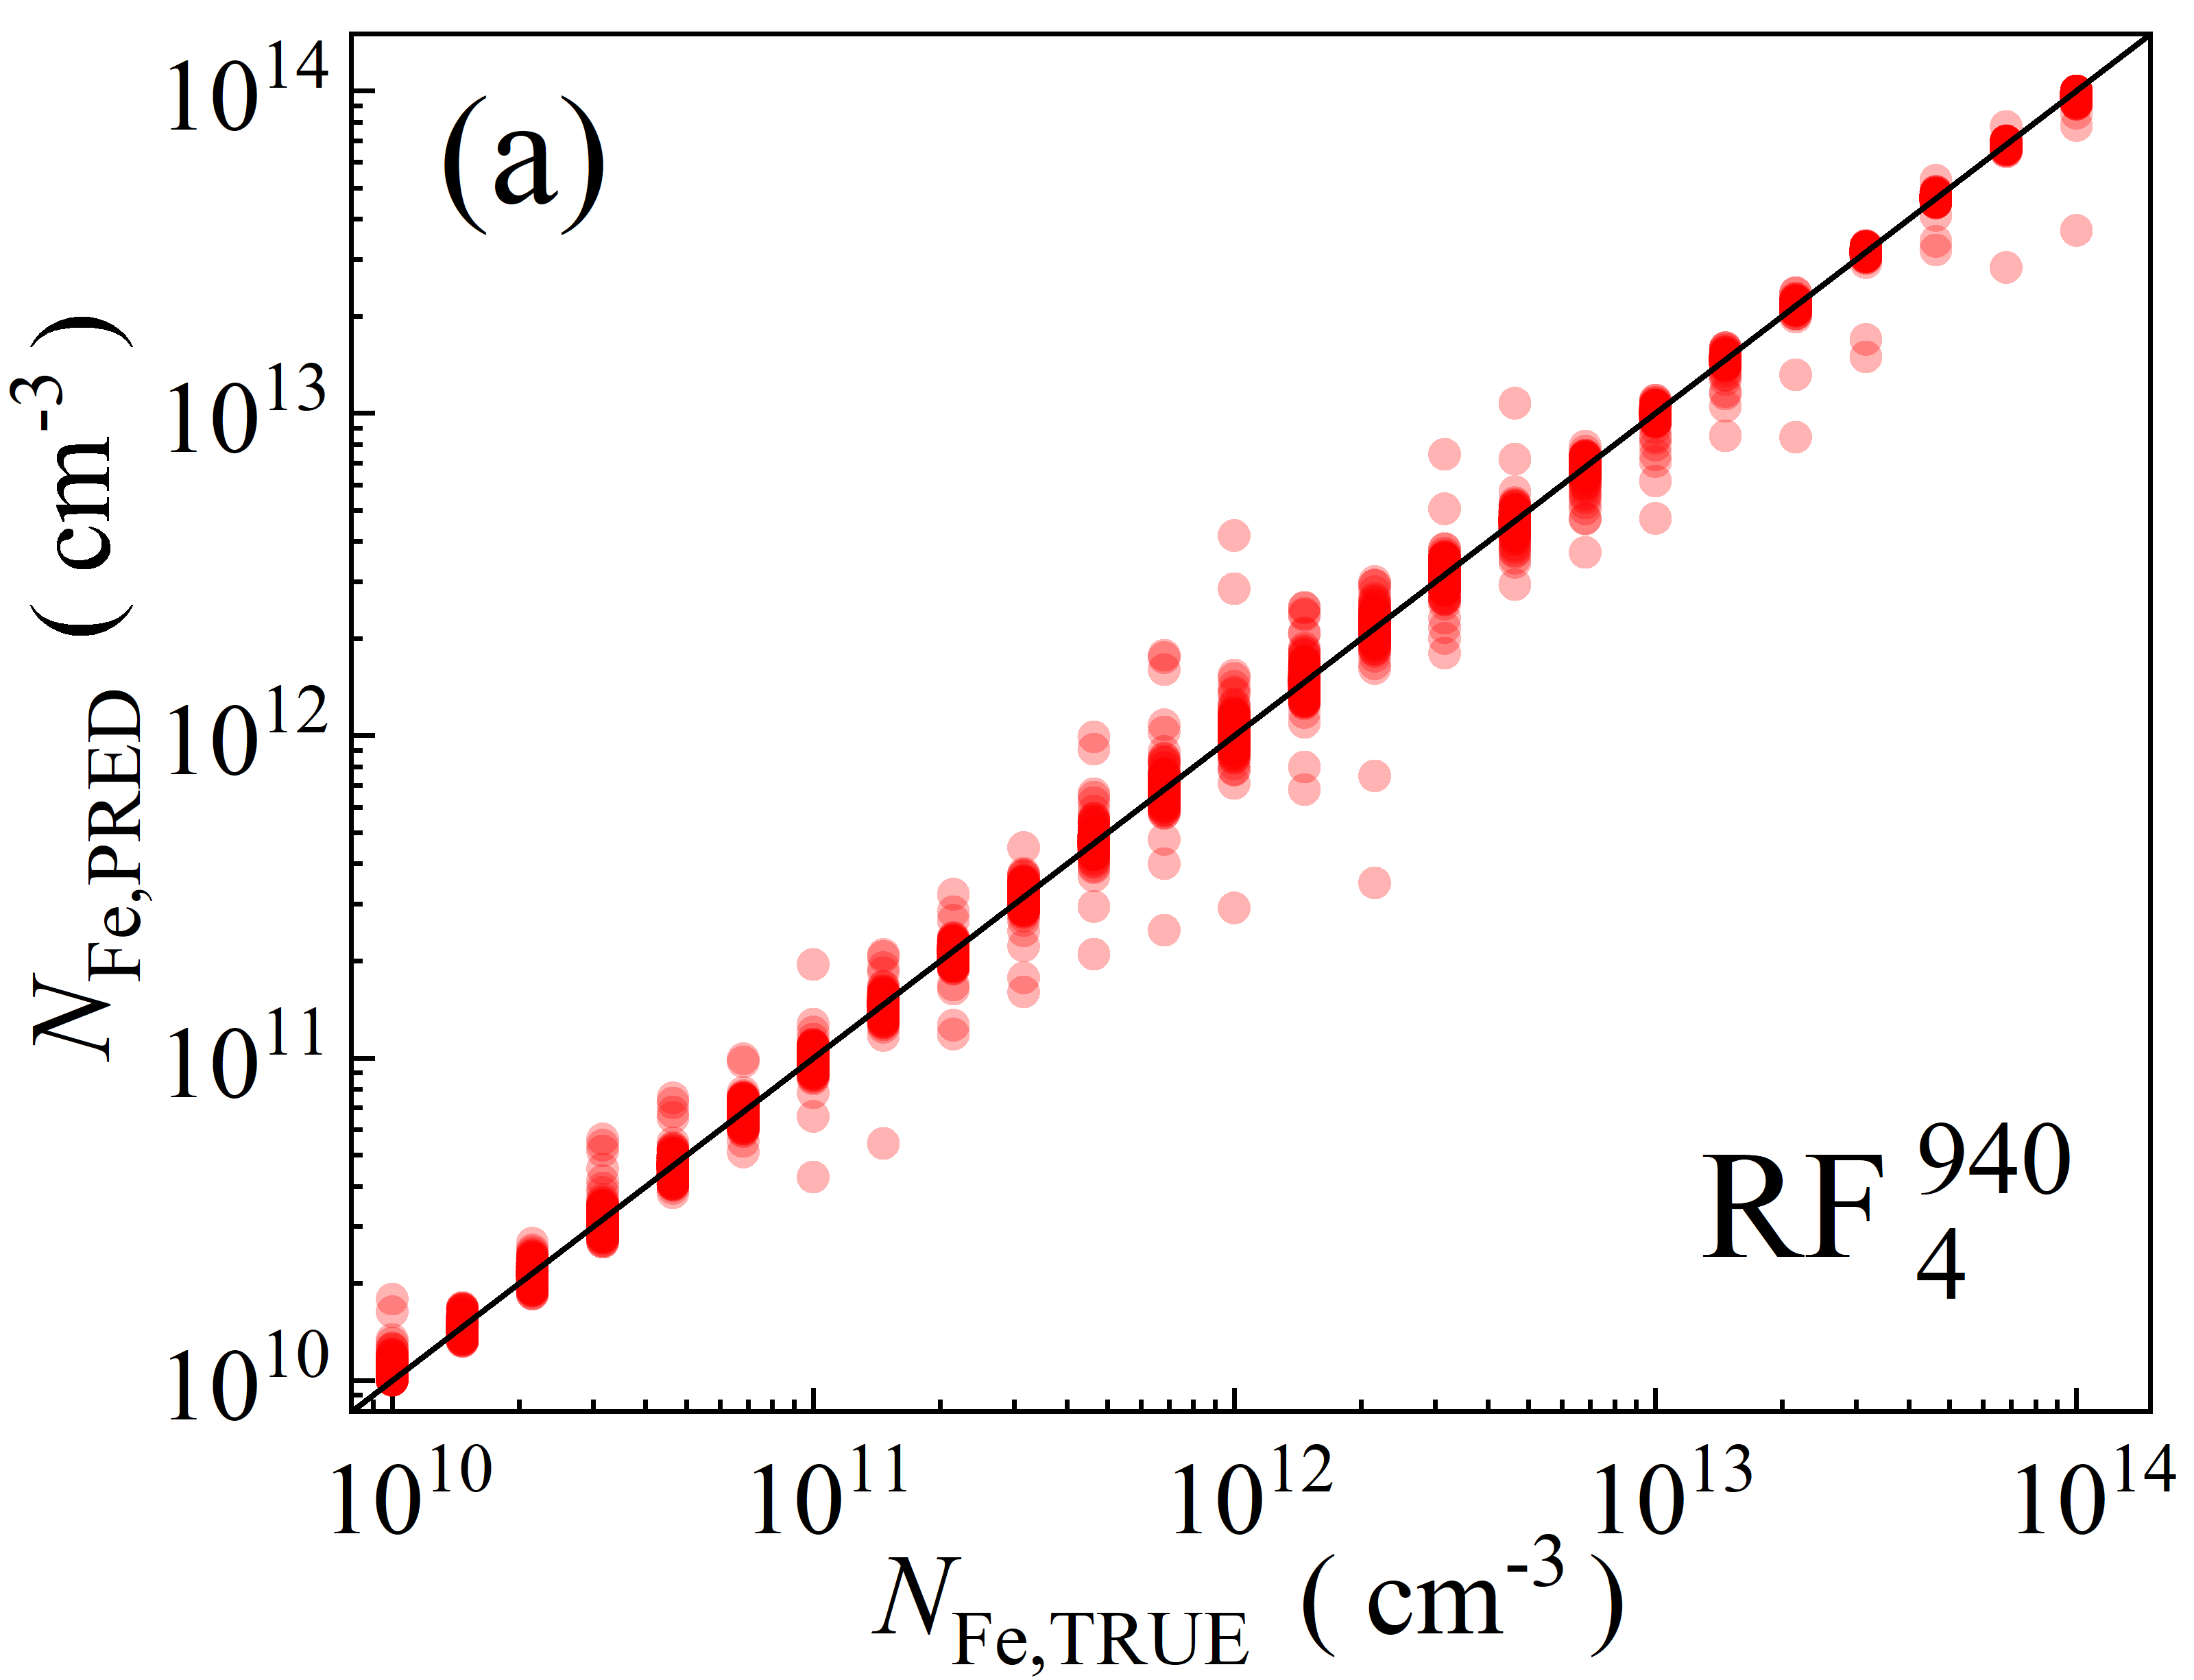
\includegraphics[width=0.4\linewidth]{Fig3a.png}
     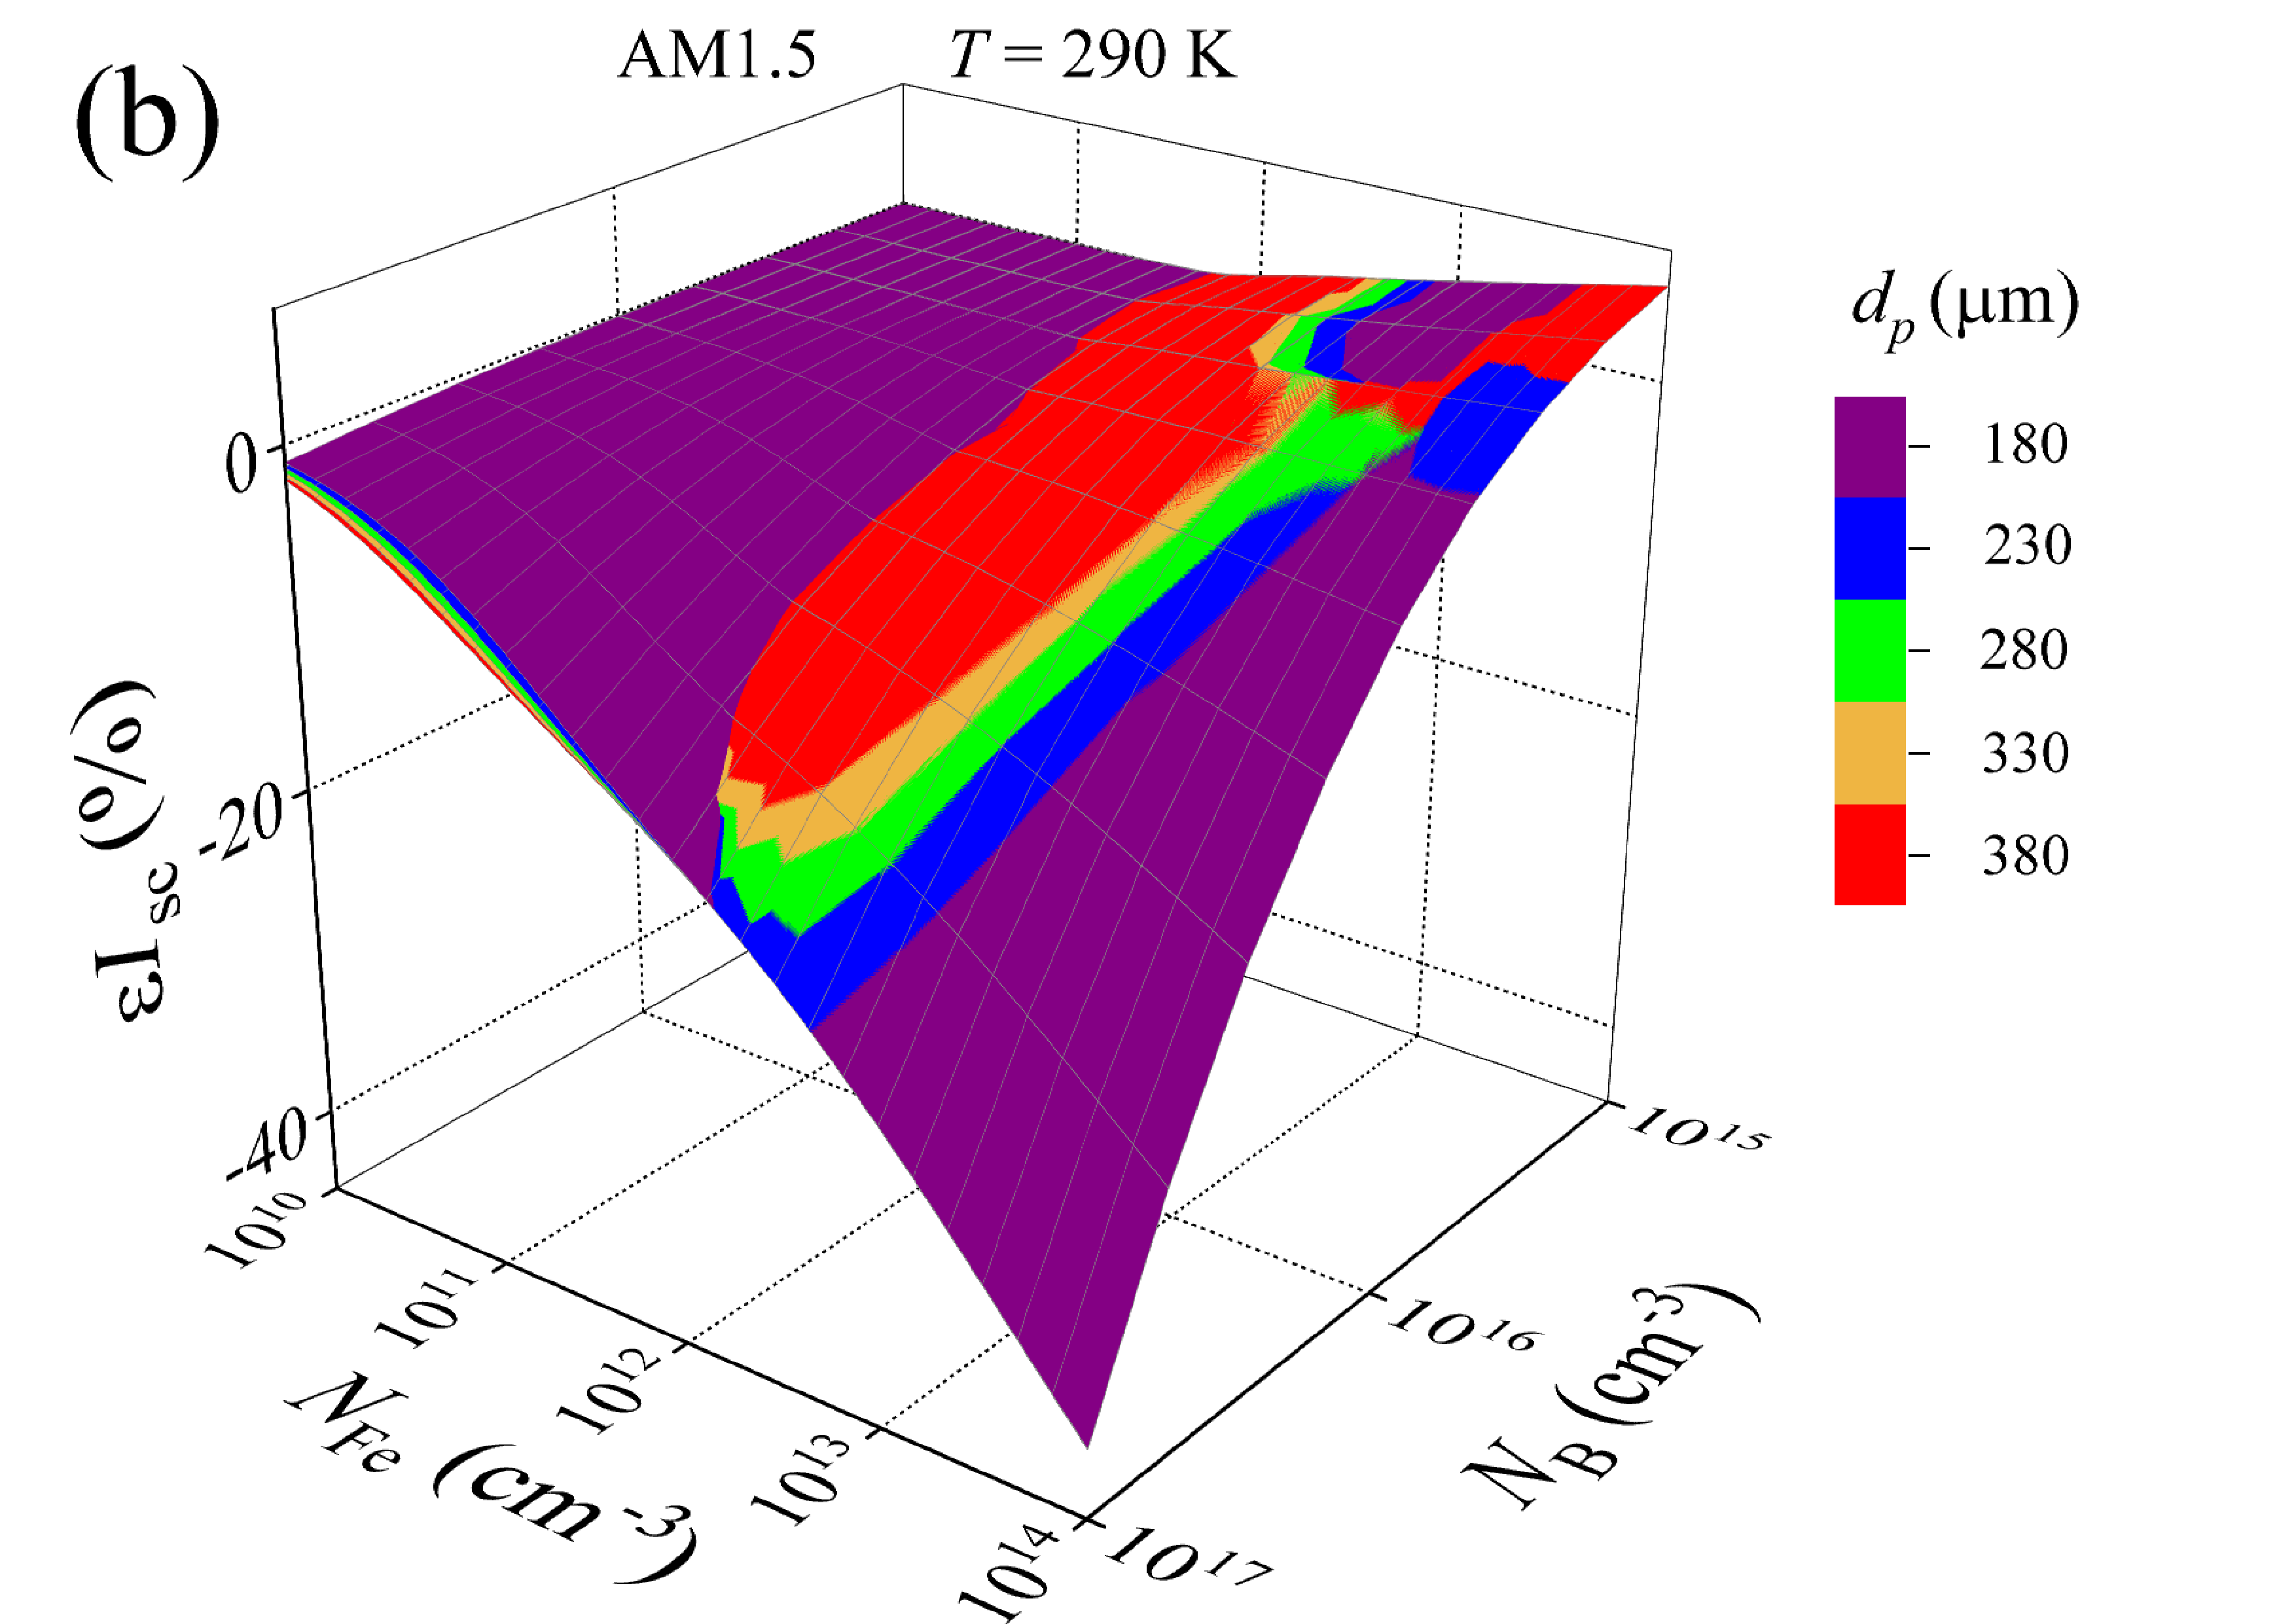
\includegraphics[width=0.4\linewidth]{Fig3b.png}
	  \caption{Dependencies of AI change in migration energy on US intensity 
      for various frequencies.
       [Fe], $10^{13}$~cm$^{-3}$: 1.0 (a), 4.2 (b).
       AW type: longitudinal (a), transverse (b).
       $T=340$~K.
       The marks are experimental results,
       the lines are the linear fitted curves.       
}\label{fig3}
\end{figure}

\begin{figure}
	\centering
     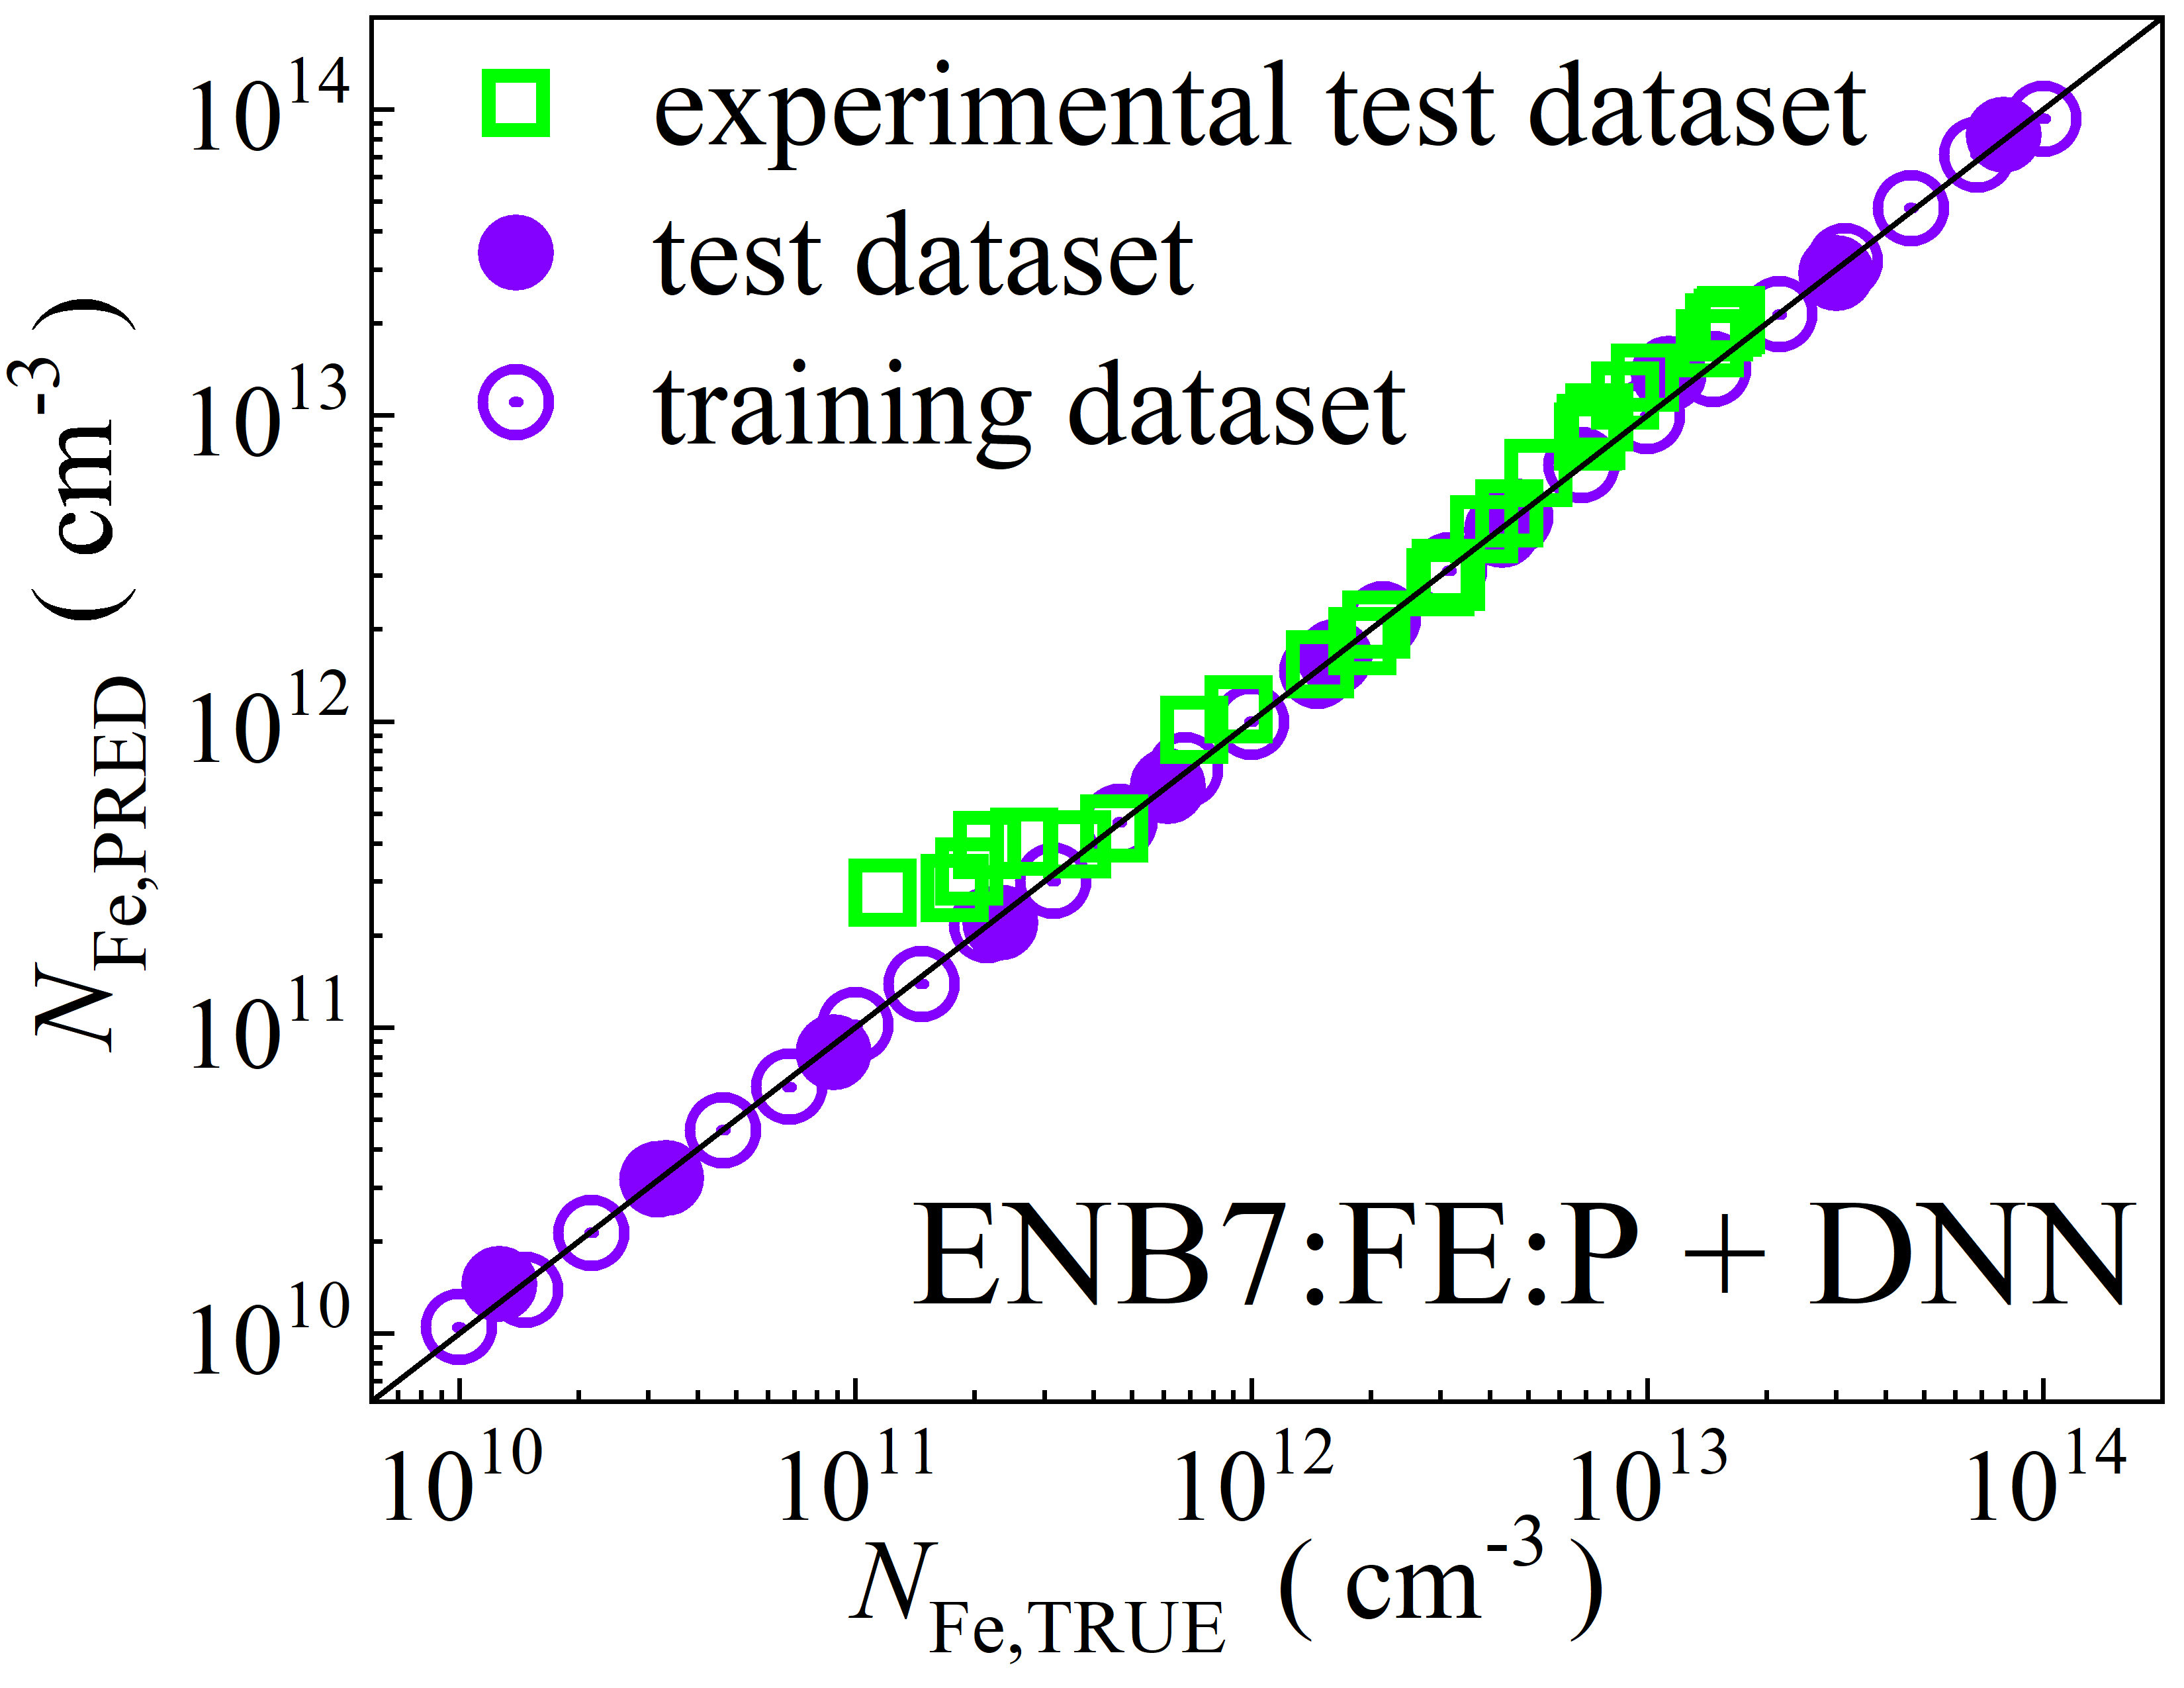
\includegraphics[width=0.4\linewidth]{Fig4a.png}
     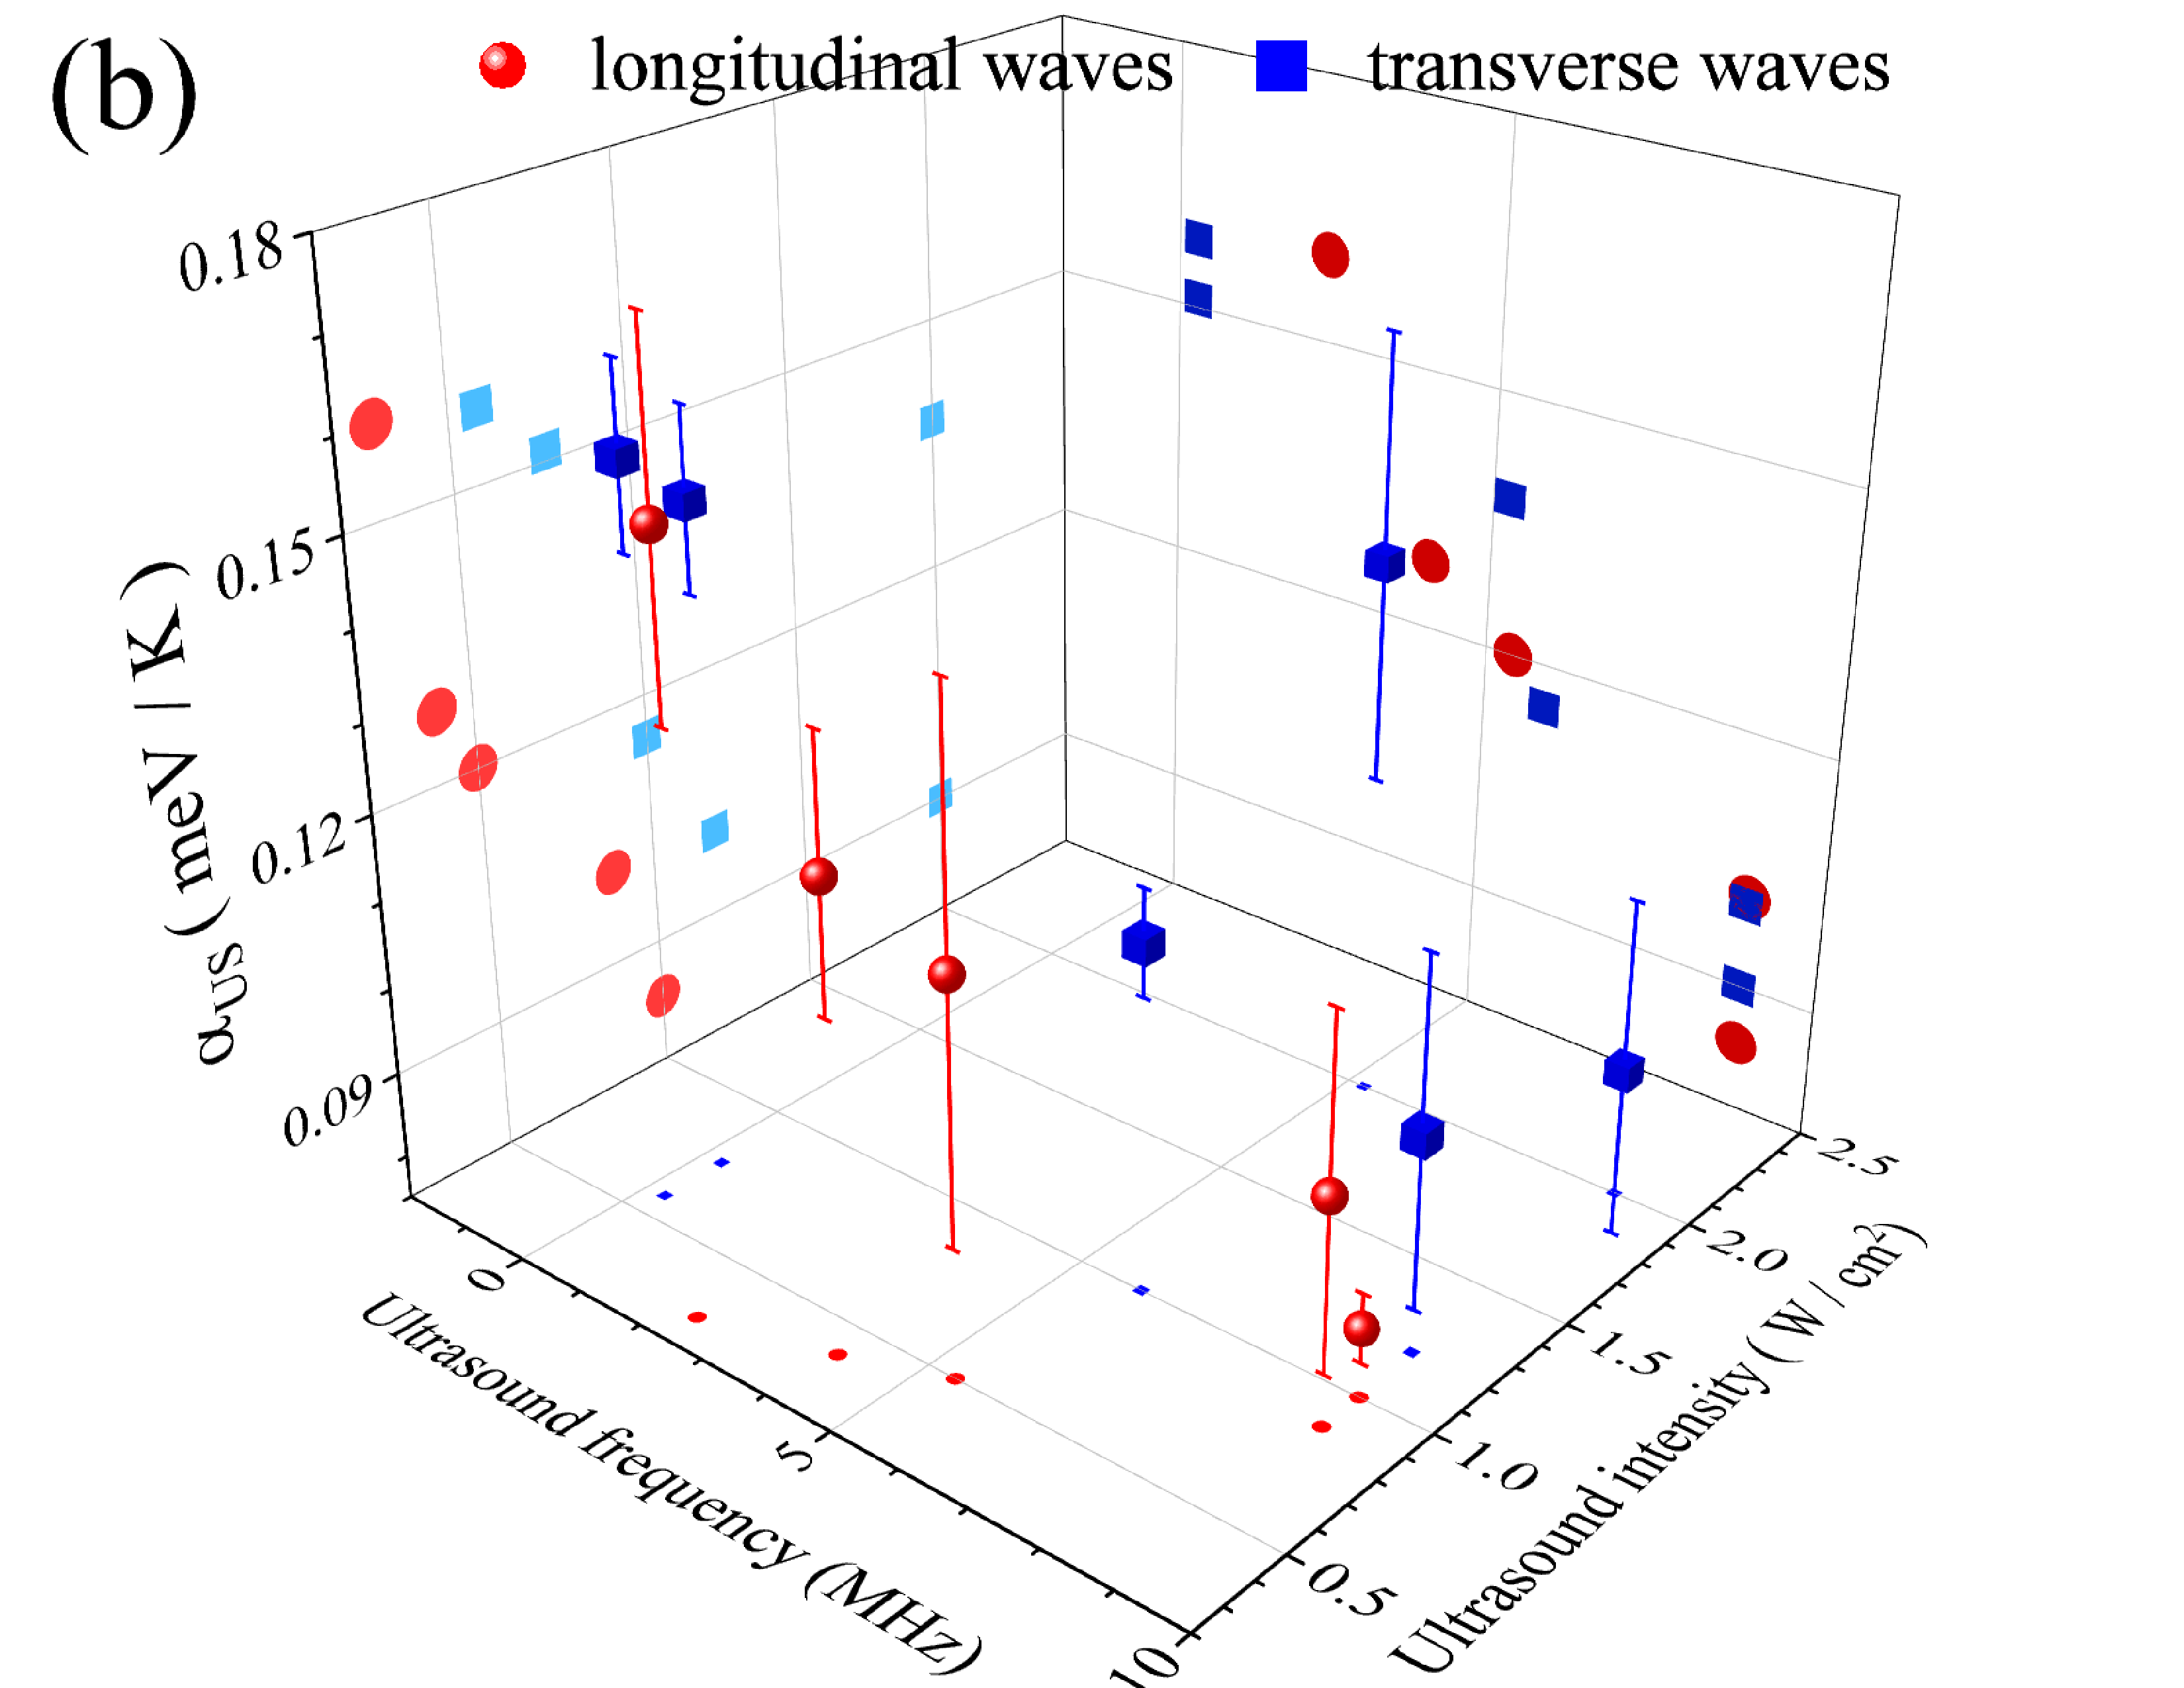
\includegraphics[width=0.4\linewidth]{Fig4b.png}
	  \caption{Dependencies of intensity coefficient (a)
       and temperature coefficient (b) of AI changes on US frequency and intensity.
       $\beta_\mathrm{US}$ values were obtained at $T=340$~K. 
       AW type: longitudinal (red circles), transverse (blue squares).
}\label{fig4}
\end{figure}

\begin{figure}
	\centering
     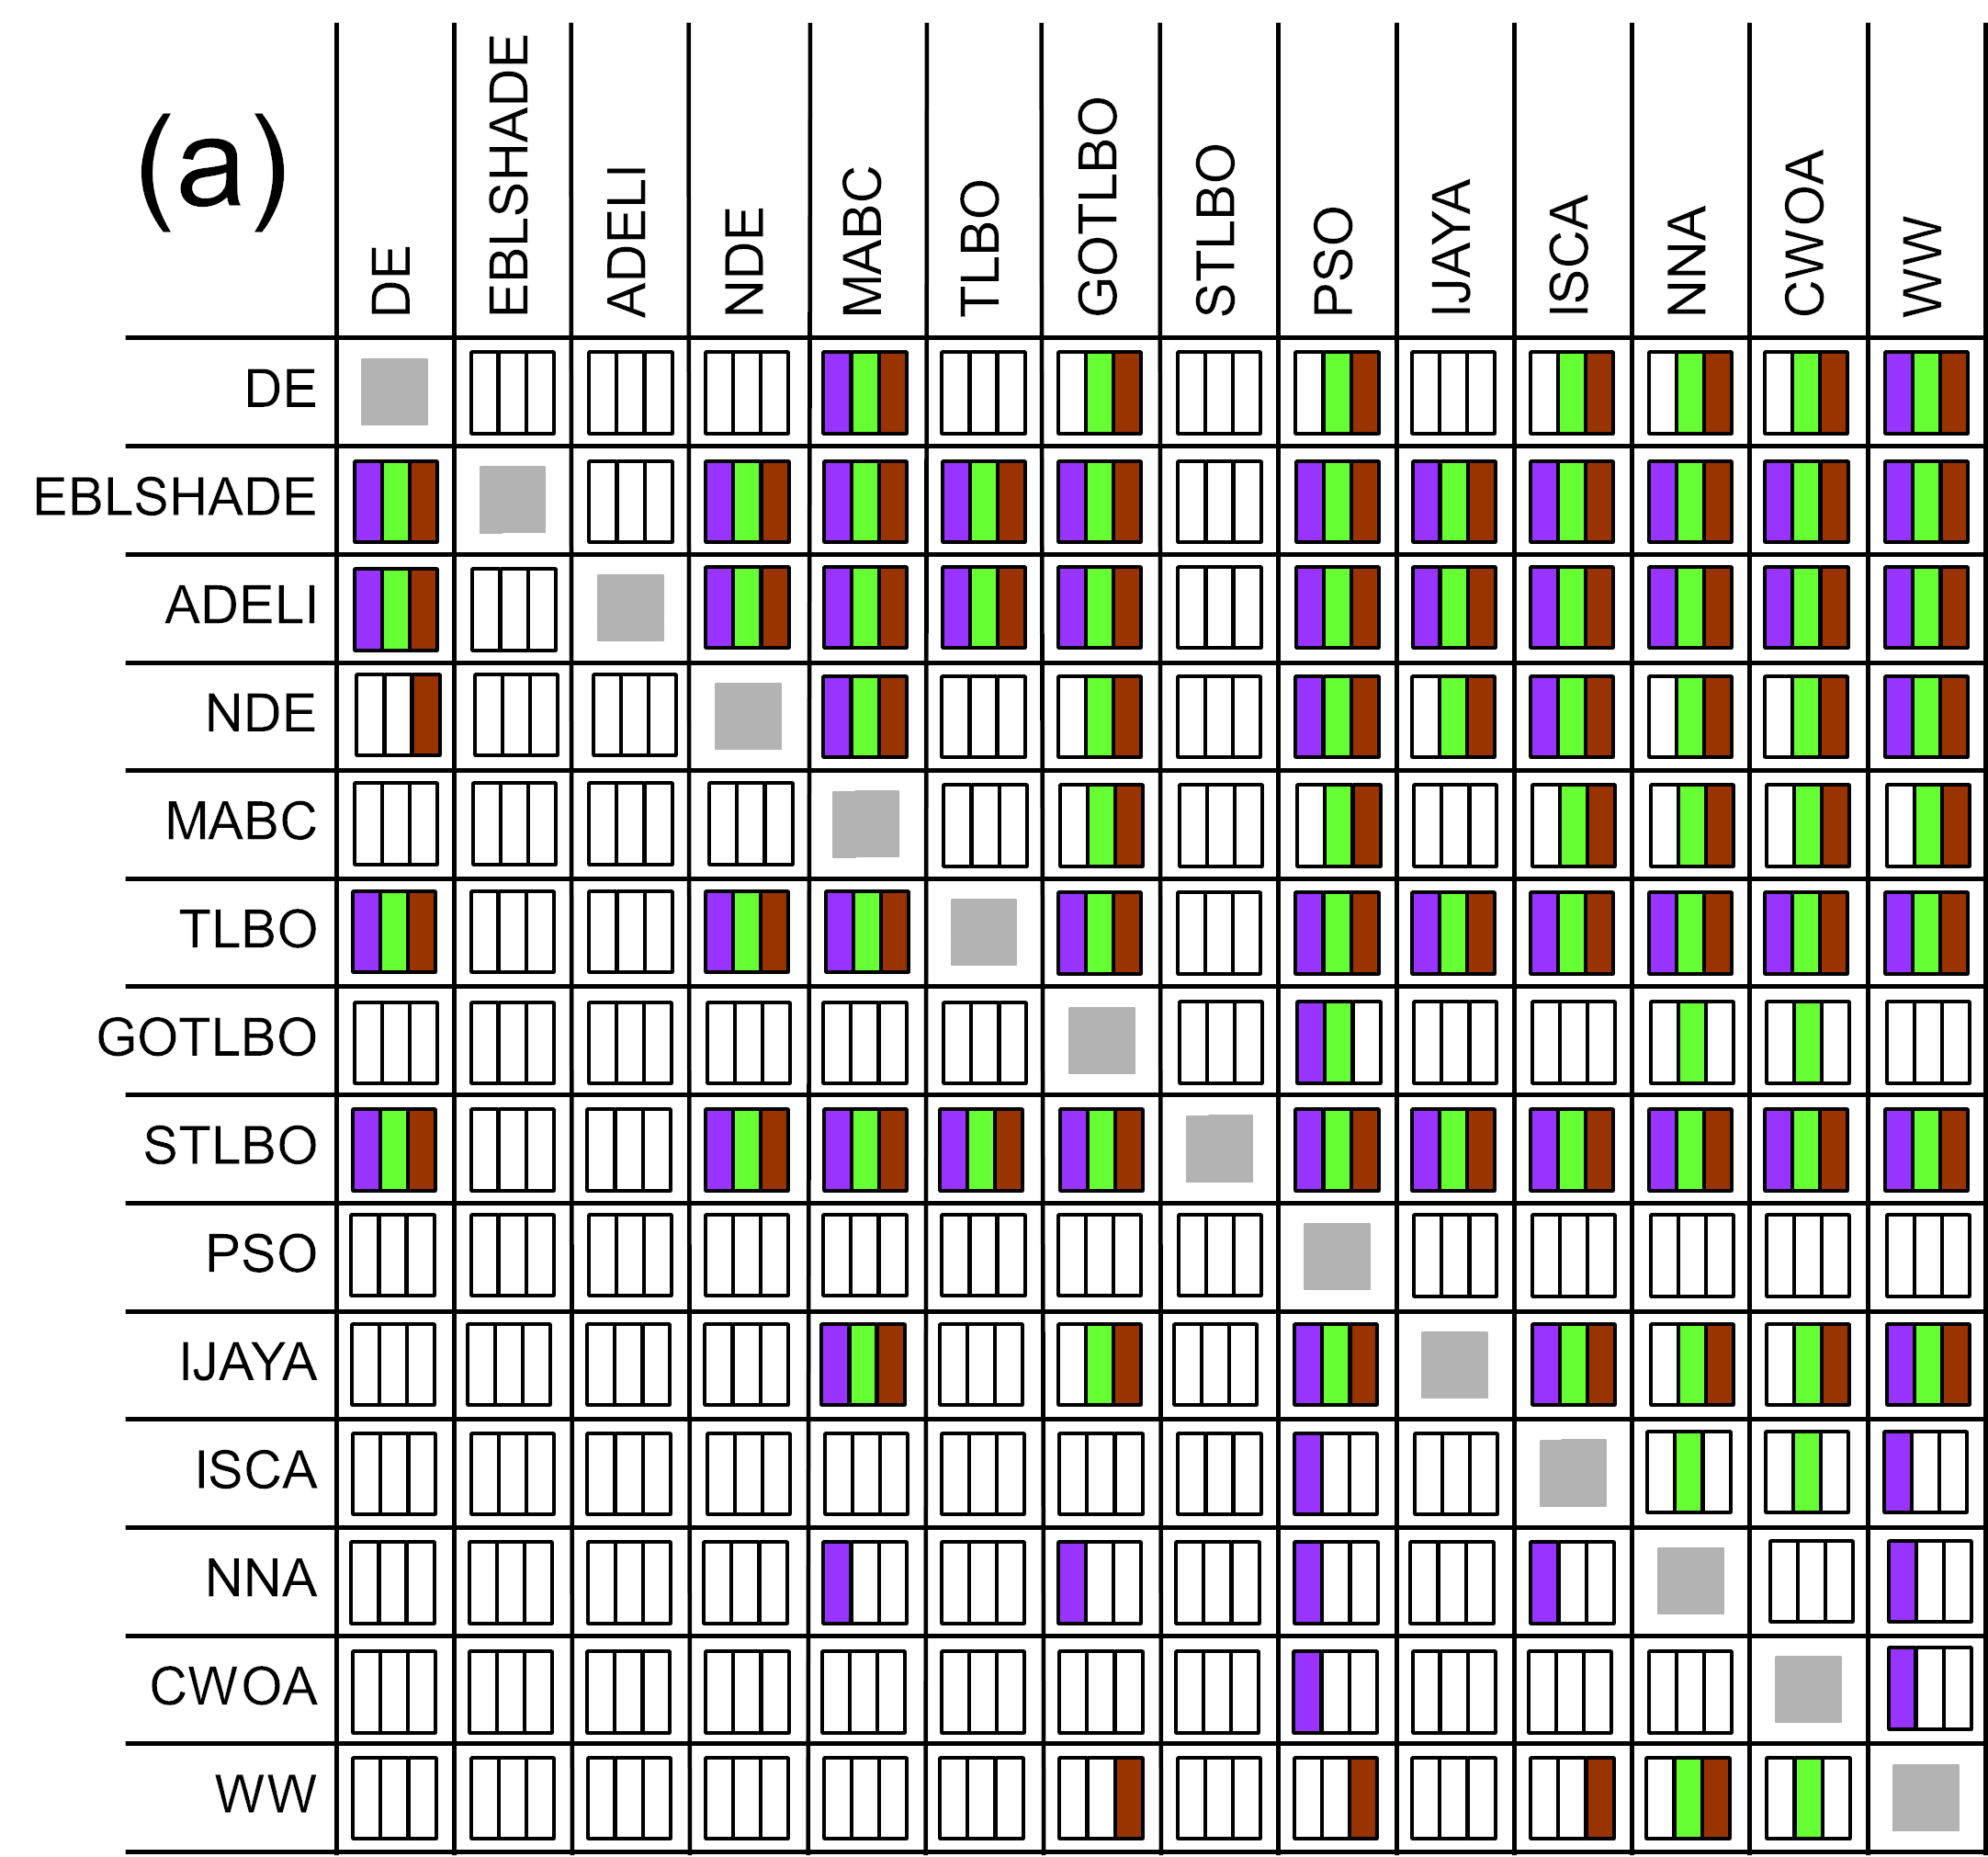
\includegraphics[width=0.4\linewidth]{Fig5a.png}
     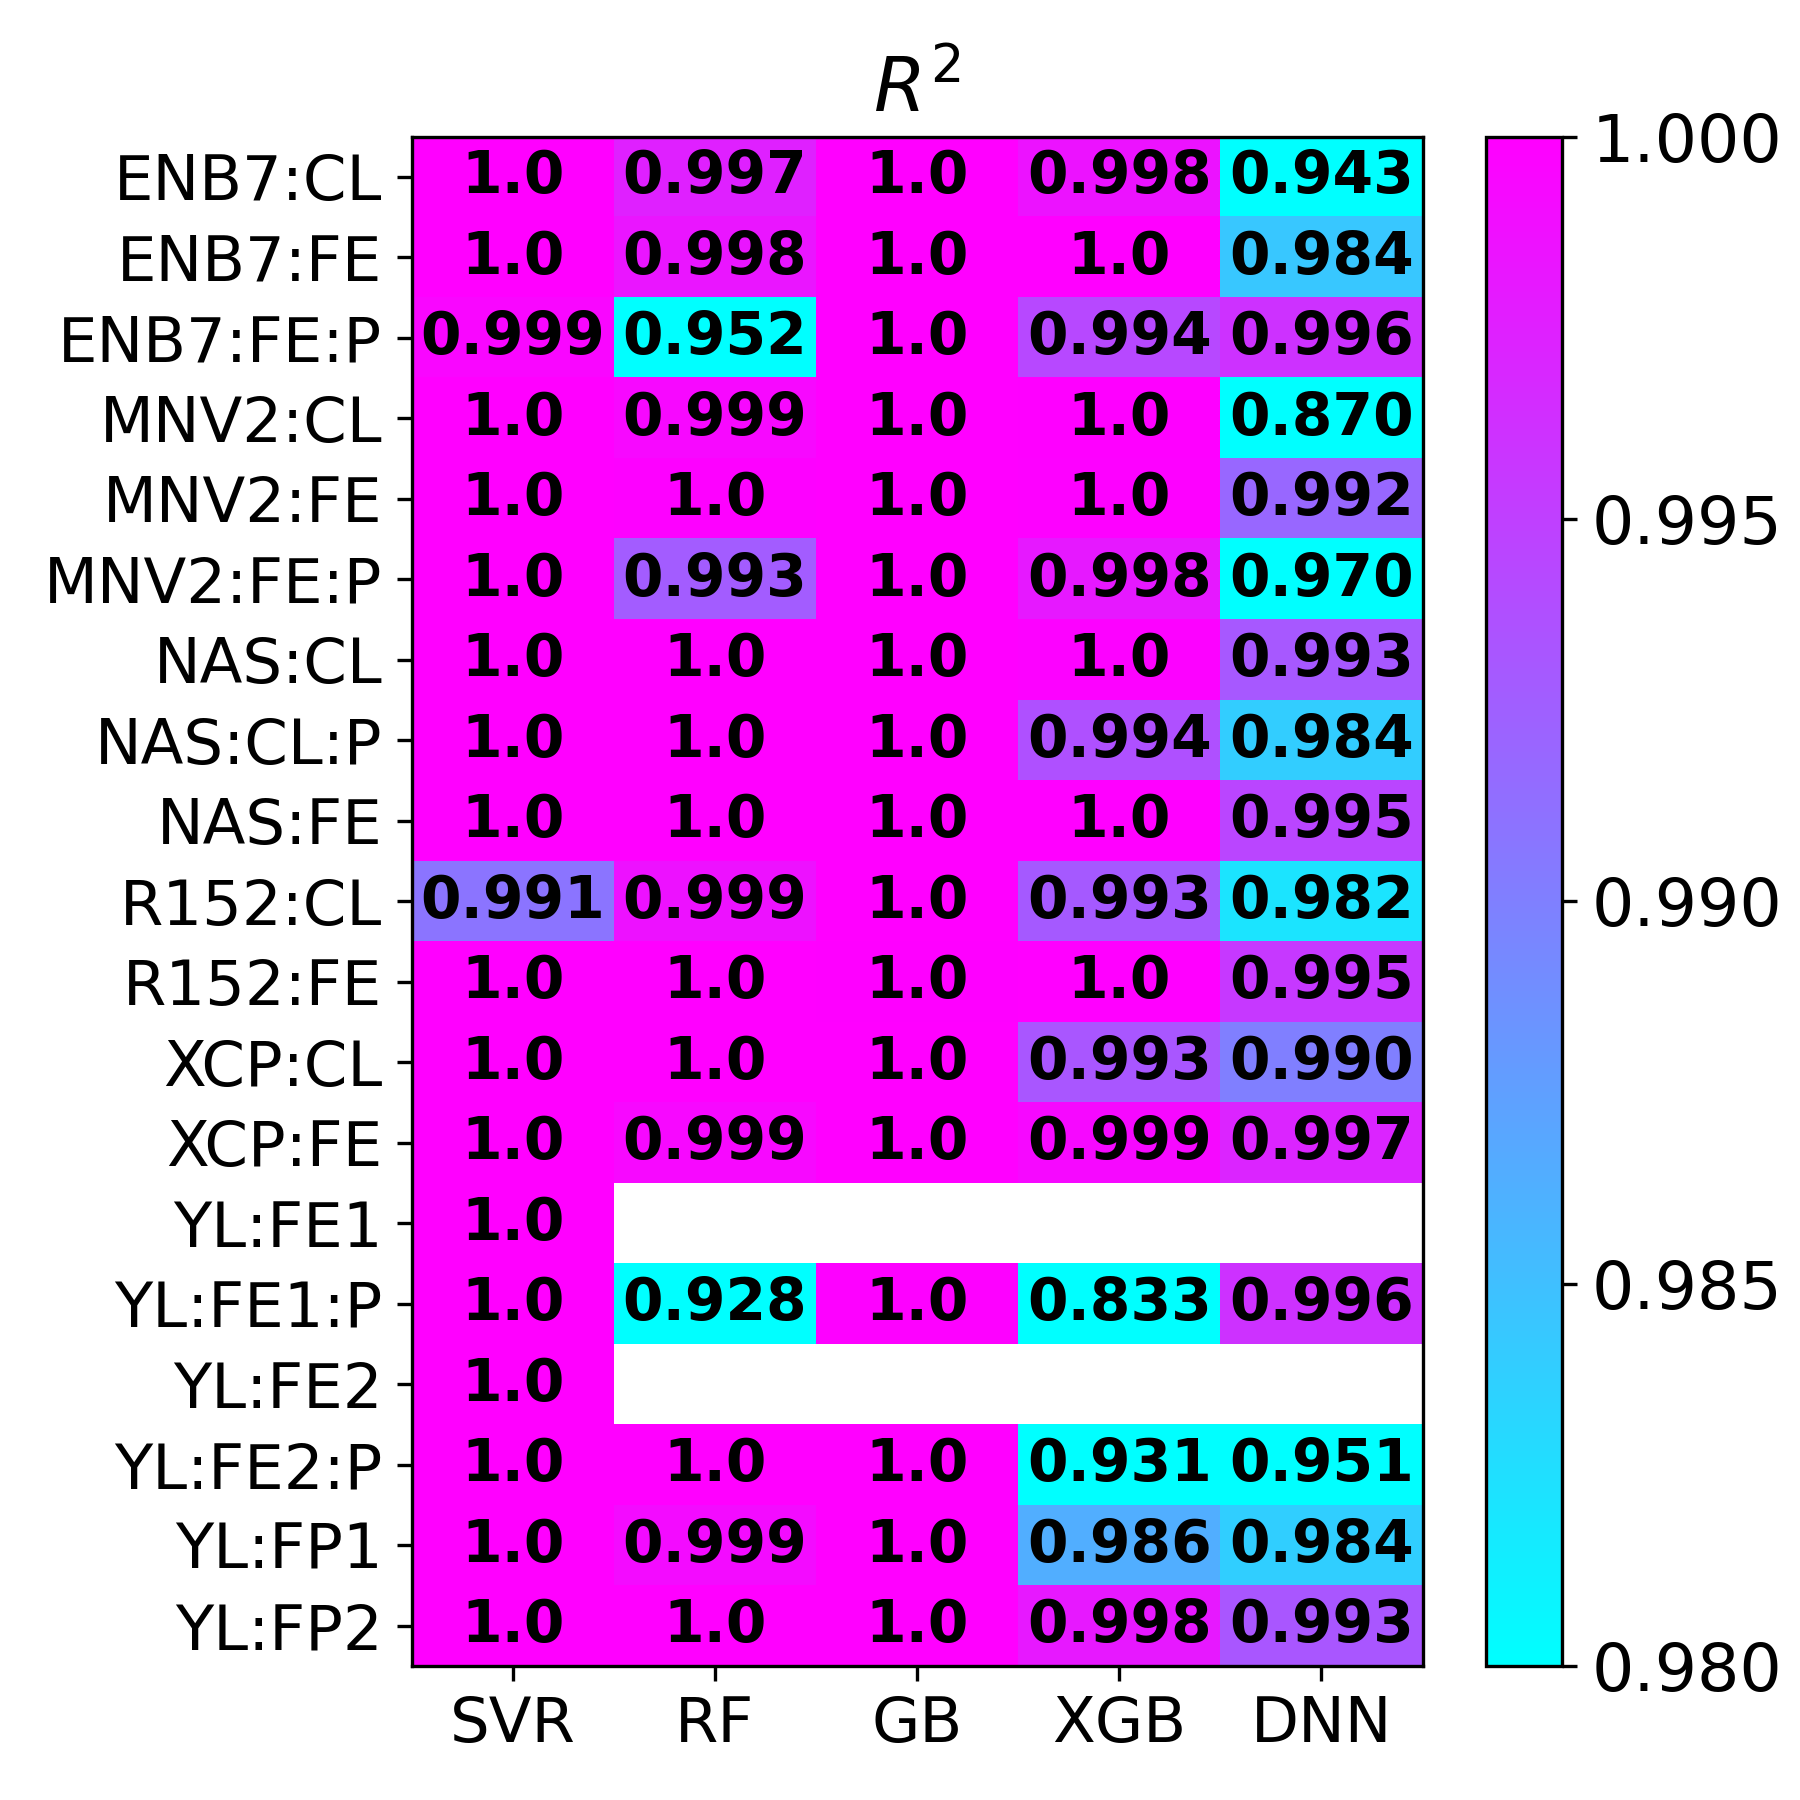
\includegraphics[width=0.4\linewidth]{Fig5b.png}
	  \caption{Temperature dependencies of $\Delta E_\mathrm{US}$.
       AW type: longitudinal (a), transverse (b).
       $f_\mathrm{US}$, MHz:  8.98 (1, 2), 5.04 (3),
       4.09 (4), 2.39 (5), 8.96 (6, 7), 5.94 (8), 5.23 (9), 0.31 (10, 11).
       $W_\mathrm{US}$, W/cm$^2$: 1.0 (1, 8), 0.87 (2), 0.1 (3), 0.4 (4), 0.3 (5), 2.0 (6, 9), 1.2 (7),
        0.76 (10), 0.58 (11).
        The marks are the experimental results, the lines are the linear fitted curves.
}\label{fig5}
\end{figure}



\section{Positron Annihilation on FeB Complex: the Searching Estimations}


\noindent \textbf{Positron Trapping.}

\noindent \textbf{Elementally-Specific Annihilaton Radiation.}

\thisfloatsetup{capposition=beside,%
      capbesideposition={right,center},
      capbesidewidth= 0.6\linewidth,
      floatwidth= 0.35\linewidth
  }

\begin{figure}
	\centering
%     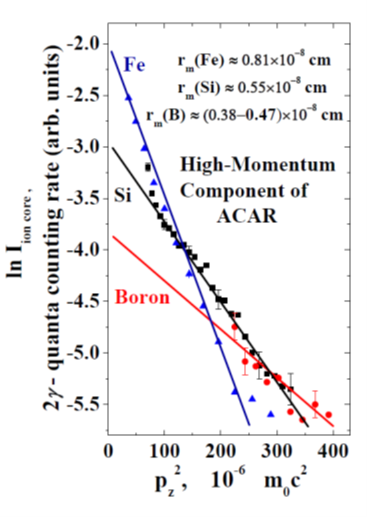
\includegraphics[width=0.35\linewidth]{Fig6.png}
     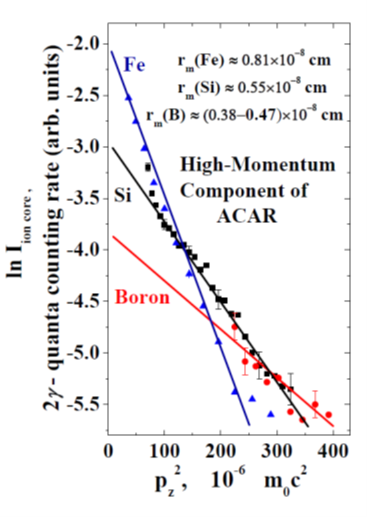
\includegraphics[width=\linewidth]{Fig6.png}
	  \caption{The high-momentum component of the elementally-specific ACAR spectra
        obtained by the spectrometer of high geometrical angular resolution $\Delta \approx 0.48 \times 10^{-3}\,m_0\,c$
        ($m_0$ and $c$ are the electron mass and the light velocity, respectively).
        The measurements were performed at room temperature and their results are given
        for boron (dots), silicon (squares), and iron (triangles).
        The electron-positron ionic radus $r_m$ were restored (see [7, 8, 9] for more detail).
        The lines are the results of fitting, the slopes of the linear functions are obtained with the accuracy
        which is characterized by the standard deviation / the Pearson’s coefficient, respectively:
        0.042/0.998 (Fe), 0.114/0.956 (B) and 0.101/0.99 (Si).
}\label{fig6}
\end{figure}

\section{Conclusion}

\section{Acknowledgments}

N. A. is thankful to DAAD for partial support of this work.
O. O. is thankful to NRFU (Pr. No. 2023.03/0252) for partial financial support of this work.

\section{References}

All manuscripts must be in English, also the table and figure texts, otherwise we cannot publish your paper.

Please keep a second copy of your manuscript in your office. When receiving the paper, we assume
that the corresponding authors grant us the copyright to use the paper for the book or journal in question.
Should authors use tables or figures from other Publications, they must ask the corresponding publishers to
grant them the right to publish this material in their paper.

Use \textit{italic} for emphasizing a word or phrase.
Do not use boldface typing or capital letters except for section headings (cf. remarks on section headings, below).


\section{Organization of the Text}


\noindent \textbf{Section Headings.} The section headings are in boldface capital and lowercase letters.
Second level headings are typed as part of the succeeding paragraph (like the subsection heading of this paragraph).

\textbf{Page Numbers.} Do \textit{not} number your paper:

\textbf{Tables.} Tables (refer with: Table 1, Table 2, ...) should be presented as part of the text, but in such a
way as to avoid confusion with the text. A descriptive title should be placed above each table. Units in tables should
 be given in square brackets [meV]. If square brackets are not available, use curly \{meV\} or standard brackets (meV).

\textbf{Special Signs}. for example , $\alpha$ $\gamma$  $\mu$ $\Omega$ () $\ge$  $\pm$ $\bullet$  $\Gamma$ \{11$\overline{2}$0\} should always be written in with the
fonts Times New Roman or Arial, especially also in the figures and tables.

\textbf{Macros}. Do not use any macros for the figures and tables. (We will not be able to convert such papers into our system)
\newpage

\textbf{Language}. All text, figures and tables must be in English.

\textbf{Figures}. Figures (refer with: Fig.~1, Fig.~2, ...) also should be presented as part of the text, leaving enough space so that the
caption will not be confused with the text. The caption should be self-contained and placed \textit{below or beside }the
figure. Generally, only original drawings or photographic reproductions are acceptable. Only very good photocopies are
acceptable. Utmost care must be taken to \textit{insert the figures in correct alignment with the text}. Half-tone pictures
 should be in the form of glossy prints. If possible, please include your figures as graphic images in the electronic version.
For best quality the pictures should have a resolution of 300 dpi(dots per inch).
\noindent Color figures are welcome for the online version of the journal. Generally, these figures will be reduced to black
and white for the print version. The author should indicate on the checklist if he wishes to have them printed in full color
and make the necessary payments in advance.

\vspace{6pt}
\textbf{Equations}.  Equations (refer with: Eq.~1, Eq.~2, ...) should be indented 5 mm (0.2").
There should be one line of space above the equation and one line of space below it before the text continues.
The equations have to be numbered sequentially, and the number put in parentheses at the right-hand edge of the
text. Equations should be punctuated as if they were an ordinary part of the text. Punctuation appears after the
equation but before the equation number, e.g.

\begin{eqnarray}
c^2 = a^2 + b^2.
\end{eqnarray}

\section{Literature References}

\noindent References are cited in the text just by square brackets [1].
 (If square brackets are not available, slashes may be used instead, e.g. /2/.)
Two or more references at a time may be put in one set of brackets [3,4]. The
references are to be numbered in the order in which they are cited in the text and
are to be listed at the end of the contribution under a heading \textit{References},
see our example below.

\section{Summary}
\noindent If you follow the `checklist` your paper will conform to the requirements
 of the publisher and facilitate a problem-free publication process.

\begin{thebibliography}{99}

\bibitem{Ostapenko1999} S. Ostapenko: Appl. Phys. A: Mater. Sci. Process. Vol. 69 (1999), p.~225

\bibitem{Ostap:PhotoLum} J. Koshka, S. Ostapenko, T. Ruf and J. M. Zhang: Appl. Phys. Lett. Vol. 69 (1996), p.~2537

\bibitem{BORKOVSKA2003} L.V. Borkovska, M.P. Baran, N.O. Korsunska et al.: Phys. B Condens. Matter Vol. 340–342 (2003), p.~258

\bibitem{Bahar2003} A. El-Bahar, S. Stolyarova, A. Chack et al.: Phys. Status Solidi A Vol. 197 (2003), p. 340

\bibitem{RITTER2008} U. Ritter, P. Scharff, V.V. Kozachenko et al.: Chem. Phys. Lett. Vol. 467 (2008), p. 77

\bibitem{Wosinski} T. Wosinski, A. Makosa and Z. Witczak: Semicond. Sci. Technol. Vol. 9 (1994), p. 2047

\bibitem{UST:OstrovCsI} I. Ostrovskii, N. Ostrovskaya, O. Korotchenkov and J. Reidy: IEEE Trans. Nucl. Sci. Vol. 52 (2005), p. 3068

\bibitem{UST:LED_SM} O. Konoreva, Ya. Olikh, M. Pinkovska et al.: Superlattices Microstruct. Vol. 102 (2017), p. 88

\bibitem{GORB2020} A.M. Gorb, O.A. Korotchenkov, O.Ya. Olikh et al.: Solid-State Electron. Vol. 165 (2020), 107712

\bibitem{Gorb2010} A.M. Gorb, O.A. Korotchenkov, O.Ya Olikh and A.O. Podolian: IEEE Trans. Nucl. Sci. Vol. 57 (2010), p. 1632

\bibitem{Litovchenko2015} V. Litovchenko, V. Melnik and B. Romanjuk: Ukrainian Journal of Physics Vol. 60 (2015), p. 64

\bibitem{ROMANJUK2005MatSci} B. Romanjuk, V. Kladko, V. Melnik et al.: Mater. Sci. Semicond. Process. Vol. 8 (2005), p. 171

\bibitem{Wang:JLum} W. Wang, F. Huang, Y. Xia and A. Wang: J. Lumin. Vol. 128 (2008), p. 199

\bibitem{US:ZnOfilm} S. Fujita, K. Kaneko, T. Ikenoue et al.: Phys. Status Solidi C. Vol. 11 (2014), p. 1225

\bibitem{YOlikhTPL2011} Ya.M. Olikh  and  M.D. Tymochko: Tech. Phys. Lett. Vol. 37 (2011), p. 37

\bibitem{Ostrovskii2001} I. Ostrovskii, O. Korotchenkov, O. Olikh et al.: J. Opt. A: Pure Appl. Opt. Vol. 3 (2001), p. S82

\bibitem{buyanova1994} I.A. Buyanova, S.S. Ostapenko, A.U. Savchuk and M.K. Sheinkman: Mater. Sci. Forum Vol. 143 (1993), p. 1063

\bibitem{belyaev1994} A.E. Belyaev, H.J. von Bardeleben, M.L. Fille et al.: Mater. Sci. Forum Vol. 143 (1993), p. 1057

\bibitem{Korotchenkov1995} O.A. Korotchenkov and H.G. Grimmliss: Phys. Rev. B. Vol. 52 (1995), p. 14598

\bibitem{Olikh2018JAP}  O.Ya. Olikh, A.M. Gorb, R.G. Chupryna and O.V. Pristay-Fenenkov: J. Appl. Phys. Vol. 123 (2018), 161573

\bibitem{Olikh:Ultras} O. Olikh: Ultrasonics Vol. 56 (2015), p. 545

\bibitem{Zaveryukhin2002} B.N. Zaveryukhin, N.N. Zaveryukhina, R.A. Muminov and O.M. Tursunkulov: Tech. Phys. Lett. Vol. 28 (2002), p. 207

\bibitem{Kuryliuk2009} V. Kuryliuk, A. Podolian and O. Korotchenkov: Cent. Eur. J. Phys. Vol. 8 (2009), p. 65

\bibitem{YOlikh:SupMicr} Ya.M. Olikh and M.D. Tymochko: Superlattices Microstruct. Vol. 95 (2016), p. 78

\bibitem{Vlasenko2000} A.I. Vlasenko,  Ya.M. Olikh  and R.K. Savkina: Semiconductors Vol. 34 (2000), p. 644

\bibitem{Gontaruk1998} A.N. Gontaruk,  D.V. Korbutyak, E.V. Korbut et al.: Tech. Phys. Lett. Vol. 24 (1999), p. 608

\bibitem{USM:Mitsumoto2014} K. Mitsumoto, M. Akatsu, S. Baba et al.: J. Phys. Soc. Jpn. Vol. 83 (2014), 034702

\bibitem{USM:SEYIDOV2016} M.Yu. Seyidov, R.A. Suleymanov, A.P. Odrinsky and C. Kırbas: Phys. B Condens. Matter Vol. 497 (2016), p. 86

\bibitem{USM:Zhevstovskikh} I.V. Zhevstovskikh, I.B. Bersuker, V.V. Gudkov et al.: J. Appl. Phys. Vol. 119 (2016), 225108

\bibitem{USM:YI2009} J. Yi, H. Kong and C. Zhu: J. Alloys Compd. Vol. 474 (2009), p. 38

\bibitem{Kor1996} O.A. Korotchenkov: Fizika i tekhnika poluprovodnikov Vol. 30 (1996), p. 1274

\bibitem{OSTROVSKII2000} I.V. Ostrovskii, O.A. Korotchenkov, R.M. Burbelo and H.G. Walther: Materials Science and Engineering: B Vol. 76 (2000), p. 139

\bibitem{SST:USmethod} I.J. Fritz and T.M. Brennan: Semicond. Sci. Technol. Vol. 12 (1997), p. 19

\bibitem{tuomisto2019} J. Slotte1, I. Makkonen and F. Tuomisto, in: Characterisation and Control of Defects 
in Semiconductors, edited by F. Tuomisto, volume 45 of Materials, Circuits and Devices, chapter,
6, Institution of Engineering \& Technology (2019).

\bibitem{FeBAssJAP2014} C. M\"{o}ller, T. Bartel, F. Gibaja and K. Lauer: J. Appl. Phys. Vol. 116 (2014), p. 024503

\bibitem{Olikh2021JAP} O. Olikh, V. Kostylyov, V. Vlasiuk et al.: J. Appl. Phys. Vol. 130 (2021), 235703

\bibitem{Olikh2022:JMatSci} O. Olikh, V. Kostylyov, V. Vlasiuk et al.: J. Mater. Sci.: Mater. Electron. Vol. 33 (2022), p. 13133

\bibitem{Pavlovich} V.N. Pavlovich:Phys. Status Solidi B Vol. 180 (1993), p. 97

\bibitem{Krevchik}  V. Krevchik, R. Muminov and A. Yafasov: Phys. Status Solidi A Vol. 632 (1981), p. K159

\bibitem{Krause1999} R. Krause-Rehberg and H.S. Leipner: \textit{Positron Annihilation in Semiconductors }(Springer–Verlag, Berlin 1999).

\bibitem{Brandt1974}W. Brandt: Appl. Phys. Vol. 5 (1974), p. 1

\bibitem{Arutyunov2013} N. Arutyunov, M. Elsayed, R. Krause-Rehberg et al.: J. Phys. Condens. Matter Vol. 25 (2013), p. 035801

\bibitem{Paudyal2009} B. Paudyal, K. Mcintosh and D. Macdonald, in: \textit{Proceedings of the 34th 
IEEE Photovoltaic Specialists Conference (PVSC)}, IEEE (2009) p. 001588.

\bibitem{Istratov1999} A. Istratov, H. Hieslmair and E. Weber: Appl. Phys. A: Mater. Sci. Process. Vol. 69 (1999), p. 13

\bibitem{Arutyunov2016}  N. Arutyunov, N. Bennett, N. Wight et al.: Phys. Status Solidi B Vol. 253 (2016), p. 2175

\bibitem{Arutyunov2006} N.Yu. Arutyunov and V.V. Emtsev: Mater. Sci. Semicond. Process. Vol. 9 (2006), p. 788

\bibitem{Arutyunov2008} N.Yu. Arutyunov and V.V. Emtsev: Mater. Sci. Semicond. Process. Vol. 11 (2008), p. 295

\bibitem{Suchet1965} J. Suchet: \textit{Chemical Physics of Semiconductors }(Van Nostrand, N.Y. 1965).

\bibitem{Rahm2016} M. Rahm, R. Hoffmann, N. W. Ashcroft: Chem. Eur. J. Vol. 22 (2016), p. 1

\bibitem{Ferrell1956} R. Ferrell:Rev. Mod. Phys. Vol. 28 (1956), p. 308

\end{thebibliography}

\end{document}